% =====================================================================
%  Prof. Fang Math — Algebra 2, 6-7 Inverse Relations & Functions
%  One source file, two PDFs:
%    pdflatex -jobname=Alg2_2-1_Domain_Range_Worksheet Alg2_2-1_Domain_Range.tex
%    pdflatex -jobname=Alg2_2-1_Domain_Range_Key "\def\iskey{1}% =====================================================================
%  Prof. Fang Math — Algebra 2, 6-7 Inverse Relations & Functions
%  One source file, two PDFs:
%    pdflatex -jobname=Alg2_2-1_Domain_Range_Worksheet Alg2_2-1_Domain_Range.tex
%    pdflatex -jobname=Alg2_2-1_Domain_Range_Key "\def\iskey{1}% =====================================================================
%  Prof. Fang Math — Algebra 2, 6-7 Inverse Relations & Functions
%  One source file, two PDFs:
%    pdflatex -jobname=Alg2_2-1_Domain_Range_Worksheet Alg2_2-1_Domain_Range.tex
%    pdflatex -jobname=Alg2_2-1_Domain_Range_Key "\def\iskey{1}% =====================================================================
%  Prof. Fang Math — Algebra 2, 6-7 Inverse Relations & Functions
%  One source file, two PDFs:
%    pdflatex -jobname=Alg2_2-1_Domain_Range_Worksheet Alg2_2-1_Domain_Range.tex
%    pdflatex -jobname=Alg2_2-1_Domain_Range_Key "\def\iskey{1}\input{Alg2_2-1_Domain_Range.tex}"
% =====================================================================
\documentclass[11pt,letterpaper]{article}
\usepackage[margin=0.8in,top=0.85in,bottom=0.8in]{geometry}
\usepackage{mathpazo}
\usepackage[T1]{fontenc}
\usepackage{amsmath,amssymb}
\usepackage{xcolor}
\usepackage{enumitem}
\usepackage{multicol}
\usepackage{booktabs}
\usepackage{needspace}
\usepackage{fancyhdr}
\usepackage[most]{tcolorbox}
\usepackage{pgfplots}
\pgfplotsset{compat=1.17}
\usetikzlibrary{arrows.meta}

\definecolor{FangBlue}{HTML}{1F4E79}
\definecolor{FangTeal}{HTML}{0F7C7C}
\definecolor{FangGold}{HTML}{C9962B}
\definecolor{FangRed}{HTML}{B3261E}
\definecolor{FangGreen}{HTML}{2E8B57}
\definecolor{FangPurple}{HTML}{6A4BD8}
\definecolor{Soft}{HTML}{F4F7FB}
% black-and-white version: pdflatex with \def\isbw{1} before \input
\ifdefined\isbw
\definecolor{FangBlue}{HTML}{000000}\definecolor{FangTeal}{HTML}{000000}\definecolor{FangGold}{HTML}{555555}
\definecolor{FangRed}{HTML}{000000}\definecolor{FangGreen}{HTML}{000000}\definecolor{FangPurple}{HTML}{000000}\definecolor{Soft}{HTML}{FFFFFF}
\fi

\newif\ifkey
\ifdefined\iskey \keytrue \else \keyfalse \fi

\pagestyle{fancy}\fancyhf{}
\renewcommand{\headrulewidth}{0.4pt}
\fancyhead[L]{\small\color{FangBlue}\textbf{Prof. Fang Math} \,|\, Algebra 2 \,·\, 2-1 Domain \& Range}
\fancyhead[R]{\small\ifkey\textcolor{FangRed}{\textbf{ANSWER KEY}}\else Name: \underline{\hspace{4.2cm}}\fi}
\fancyfoot[C]{\small\thepage}
\fancyfoot[R]{\scriptsize\color{gray}fangmath.com}
\setlength{\headheight}{14pt}
\setlength{\parindent}{0pt}
\setlength{\parskip}{4pt}

% ---------- boxes ----------
\newtcolorbox{idea}[1][]{colback=Soft,colframe=FangBlue,boxrule=0.8pt,arc=3pt,left=8pt,right=8pt,top=6pt,bottom=6pt,
  fonttitle=\bfseries,coltitle=white,colbacktitle=FangBlue,title={#1}}
\newtcolorbox{example}[1][]{colback=white,colframe=FangTeal,boxrule=0.6pt,arc=3pt,left=8pt,right=8pt,top=5pt,bottom=5pt,
  fonttitle=\bfseries,coltitle=FangTeal,colbacktitle=white,title={#1},attach boxed title to top left={xshift=8pt,yshift=-7pt},boxed title style={boxrule=0pt,colframe=white}, enhanced}
\newtcolorbox{warn}{colback=FangRed!5,colframe=FangRed,boxrule=0.6pt,arc=3pt,left=8pt,right=8pt,top=4pt,bottom=4pt,leftrule=3pt}
\newtcolorbox{simple}{colback=FangGold!10,colframe=FangGold,boxrule=0.6pt,arc=3pt,left=8pt,right=8pt,top=4pt,bottom=4pt,leftrule=3pt}
\newtcolorbox{sol}{colback=FangGreen!6,colframe=FangGreen,boxrule=0.5pt,arc=2pt,left=6pt,right=6pt,top=3pt,bottom=3pt,breakable}

\newcommand{\badge}[2]{\tcbox[on line,colback=#1,colframe=#1,coltext=white,boxrule=0pt,arc=6pt,left=4pt,right=4pt,top=1pt,bottom=1pt,fontupper=\scriptsize\bfseries]{#2}}
\newcommand{\easy}{\badge{FangGreen}{EASY}}
\newcommand{\medium}{\badge{FangTeal}{MEDIUM}}
\newcommand{\hard}{\badge{FangRed}{HARD}}
\newcommand{\work}[2][]{\ifkey\begin{sol}#2\end{sol}\else\vspace*{#1}\fi}
\newcommand{\np}[1][6cm]{\needspace{#1}}
\newcommand{\sect}[2]{\par\needspace{7cm}\medskip{\Large\bfseries\color{FangBlue}\tcbox[on line,colback=FangBlue,colframe=FangBlue,coltext=white,arc=2pt,boxrule=0pt,left=5pt,right=5pt,top=1pt,bottom=1pt]{#1}\ #2}\par\smallskip}


\newcommand{\R}{\mathbb{R}}
% small graph for practice problems: \gr{plot commands}
\newcommand{\gr}[2][]{\begin{tikzpicture}\begin{axis}[width=5.0cm,height=5.0cm,axis lines=middle,xmin=-6,xmax=6,ymin=-6,ymax=6,
  xtick={-4,-2,2,4},ytick={-4,-2,2,4},grid=both,minor tick num=1,grid style={gray!18},major grid style={gray!30},
  xlabel={\scriptsize$x$},ylabel={\scriptsize$y$},tick label style={font=\tiny},clip=true,#1]#2\end{axis}\end{tikzpicture}}
\newcommand{\opn}[2]{\draw[FangBlue,thick,fill=white](axis cs:#1,#2) circle(2.4pt);}
\newcommand{\cls}[2]{\fill[FangBlue](axis cs:#1,#2) circle(2.4pt);}

\begin{document}

% ======================= TITLE =======================
\begin{center}
{\color{FangBlue}\Huge\bfseries Domain \& Range}\\[2pt]
{\large What can go in? What can come out?}
\ifkey\\[3pt]{\color{FangRed}\large\bfseries Answer Key with complete solutions}\fi
\end{center}
\vspace{-4pt}

\begin{idea}[The big idea]
A function is a machine: you put in an $x$, it gives back one $y$.
\begin{itemize}[leftmargin=*,itemsep=1pt,topsep=2pt]
\item The \textbf{domain} is every $x$ you are \textbf{allowed to put in}. \quad (inputs, the horizontal direction)
\item The \textbf{range} is every $y$ that can \textbf{actually come out}. \quad (outputs, the vertical direction)
\end{itemize}
\end{idea}

\begin{simple}
\textbf{Simple case first.} For $f(x)=\sqrt{x}$, try a few inputs: $f(9)=3$, $f(0)=0$, but $f(-4)$ is not a real number. So the domain is $x\ge0$. And since a square root is never negative, the outputs are $y\ge0$. Testing a few easy numbers is always a good way to start.
\end{simple}

% ======================= PART 1 =======================
\sect{1}{Three ways to write a set of numbers}

\begin{center}
\renewcommand{\arraystretch}{1.35}
\begin{tabular}{@{}llll@{}}
\toprule
\textbf{In words} & \textbf{Inequality} & \textbf{Interval notation} & \textbf{Set-builder}\\ \midrule
from $-2$ to $5$, including $-2$, not $5$ & $-2\le x<5$ & $[-2,\,5)$ & $\{x\mid -2\le x<5\}$\\
greater than $3$ & $x>3$ & $(3,\,\infty)$ & $\{x\mid x>3\}$\\
at most $-1$ & $x\le -1$ & $(-\infty,\,-1]$ & $\{x\mid x\le-1\}$\\
all real numbers & — & $(-\infty,\,\infty)$ & $\R$\\
every number except $2$ & $x\neq2$ & $(-\infty,2)\cup(2,\infty)$ & $\{x\mid x\neq 2\}$\\
\bottomrule
\end{tabular}
\end{center}

\begin{multicols}{2}
\textbf{Square bracket} $[\ ]$: the endpoint is \textbf{included} (closed dot $\bullet$, $\le$ or $\ge$).\par
\textbf{Parenthesis} $(\ )$: the endpoint is \textbf{not included} (open dot $\circ$, $<$ or $>$).
\columnbreak

$\infty$ is not a number you can reach, so it \textbf{always} gets a parenthesis.\par
$\cup$ means ``or'' — it joins two pieces.
\end{multicols}

% ======================= PART 2 =======================
\sect{2}{From points, a table, or a mapping}

\begin{example}[Example 1]
$\{(-1,4),\ (0,2),\ (3,4),\ (5,-1)\}$ \qquad Domain: list the $x$'s: $\{-1,0,3,5\}$. \quad Range: list the $y$'s: $\{-1,2,4\}$.\par
List each value \textbf{once}, from smallest to largest ($4$ appears twice but is written once).
\end{example}

% ======================= PART 3 =======================
\sect{3}{From a graph: look at the shadows}

\begin{minipage}[t]{0.5\textwidth}\vspace{0pt}\centering
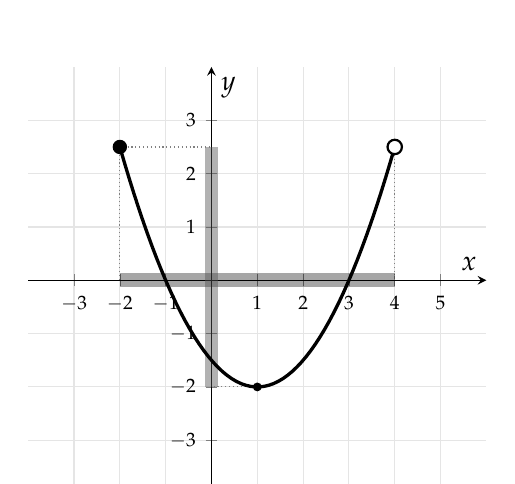
\begin{tikzpicture}
\begin{axis}[width=7.4cm,height=7cm,axis lines=middle,xmin=-4,xmax=6,ymin=-4,ymax=4,
  xtick={-3,-2,-1,1,2,3,4,5},ytick={-3,-2,-1,1,2,3},grid=major,grid style={gray!20},
  xlabel={$x$},ylabel={$y$},tick label style={font=\scriptsize}]
\draw[FangTeal,line width=5pt,opacity=0.35](axis cs:-2,0)--(axis cs:4,0);
\draw[FangGold,line width=5pt,opacity=0.45](axis cs:0,-2)--(axis cs:0,2.5);
\draw[densely dotted,gray](axis cs:-2,2.5)--(axis cs:-2,0);
\draw[densely dotted,gray](axis cs:4,2.5)--(axis cs:4,0);
\draw[densely dotted,gray](axis cs:-2,2.5)--(axis cs:0,2.5);
\draw[densely dotted,gray](axis cs:1,-2)--(axis cs:0,-2);
\addplot[FangBlue,very thick,domain=-2:4,samples=60]{0.5*(x-1)^2-2};
\fill[FangBlue](axis cs:-2,2.5) circle(2.6pt);
\draw[FangBlue,thick,fill=white](axis cs:4,2.5) circle(2.6pt);
\fill[FangBlue](axis cs:1,-2) circle(1.6pt);
\end{axis}
\end{tikzpicture}
\end{minipage}\hfill
\begin{minipage}[t]{0.47\textwidth}\vspace{4pt}
Shine a light from above: the graph's \textbf{shadow on the $x$-axis} (teal) is the \textbf{domain}. Shine it from the side: the \textbf{shadow on the $y$-axis} (gold) is the \textbf{range}.

\textbf{Read the domain} left to right: from $x=-2$ (closed dot, included) to $x=4$ (open dot, not included):
\[\text{Domain} = [-2,\,4).\]
\textbf{Read the range} bottom to top: the lowest point is the vertex, $y=-2$. The highest $y$ is $2.5$ — the open dot does \emph{not} reach it, but the closed dot at $(-2,\,2.5)$ does:
\[\text{Range} = [-2,\,2.5].\]
\end{minipage}

\begin{warn}
\textbf{Watch out:} an \textbf{arrow} means the graph keeps going, so that side goes to $\infty$ or $-\infty$. An open dot only leaves out that \emph{one point} — check whether another part of the graph reaches the same $y$.
\end{warn}

% ======================= PART 4 =======================
\sect{4}{From an equation: what could go wrong?}

\begin{idea}[Domain: start with all real numbers, then remove only what breaks]
\begin{tabular}{@{}lll@{}}
\textbf{1. Division by zero} & a denominator can't be $0$ & $\dfrac{1}{x-3}$: \ $x\neq3$\\[8pt]
\textbf{2. Even roots of negatives} & what is under $\sqrt{\ }$ must be $\ge0$ & $\sqrt{x+5}$: \ $x\ge-5$\\[4pt]
\textbf{3. Real-world limits} & time, length, people can't be negative & $t\ge0$, $n$ a whole number
\end{tabular}\par\smallskip
Nothing else breaks: polynomials, absolute value and \textbf{odd} roots like $\sqrt[3]{x}$ have domain $\R$.
\end{idea}

\textbf{Range: where can the outputs go?} Use the shape of the graph.

\begin{center}
\renewcommand{\arraystretch}{1.3}
\begin{tabular}{@{}lll@{}}
\toprule
\textbf{Function} & \textbf{Look at\ldots} & \textbf{Range}\\ \midrule
$a(x-h)^2+k$ & the vertex $(h,k)$: up if $a>0$, down if $a<0$ & $[k,\infty)$ or $(-\infty,k]$\\
$a\sqrt{x-h}+k$ & the starting point $(h,k)$ & $[k,\infty)$ if $a>0$, \ $(-\infty,k]$ if $a<0$\\
$a|x-h|+k$ & the vertex $(h,k)$ & $[k,\infty)$ or $(-\infty,k]$\\
$\dfrac{a}{x-h}+k$ & the horizontal asymptote $y=k$ & every $y$ except $k$\\
$mx+b$, \ $m\neq0$ & — & $\R$\\
\bottomrule
\end{tabular}
\end{center}

\begin{example}[Example 2 \;·\; a quadratic in standard form]
$f(x)=-x^2+6x-5$. \ Domain: a polynomial, so $\R$. \par
Vertex: $x=-\frac{b}{2a}=-\frac{6}{-2}=3$, and $f(3)=-9+18-5=4$. It opens down ($a<0$), so the highest output is $4$:
\quad Range $=(-\infty,\,4]$.
\end{example}

\begin{example}[Example 3 \;·\; a square root]
$g(x)=\sqrt{2x-6}+1$. \ Domain: $2x-6\ge0 \Rightarrow x\ge3$, so $[3,\infty)$.\par
Range: the square root starts at $0$ and grows, so $g$ starts at $0+1=1$ and grows: $[1,\infty)$. \ Simple case check: $g(3)=1$, $g(5)=3$. \checkmark
\end{example}

\begin{example}[Example 4 \;·\; a rational function — solve for $x$ to find the range]
$h(x)=\dfrac{2x+1}{x-4}$. \ Domain: $x\neq4$.\par
Range: set $y=\dfrac{2x+1}{x-4}$ and solve for $x$: \ $yx-4y=2x+1 \Rightarrow x(y-2)=4y+1 \Rightarrow x=\dfrac{4y+1}{y-2}$.\par
This works for every $y$ \textbf{except} $y=2$. So Range $=\{y\mid y\neq2\}$ — the horizontal asymptote.
\end{example}

\begin{warn}
\textbf{Common mistakes:} (1) Writing the domain of $\sqrt{x-4}$ as $x>4$ — it is $x\ge4$, because $\sqrt0=0$ is fine. \ (2) Saying the domain of $\frac{1}{x^2+1}$ excludes something — $x^2+1$ is never $0$, so the domain is $\R$. \ (3) Mixing up domain ($x$) and range ($y$).
\end{warn}

% ======================= PRACTICE =======================
\newpage
\sect{5}{Practice}
\ifkey\else\textit{Write every answer in interval notation (or as a list for sets of points). Test one or two easy numbers to check.}\fi

\medskip
\needspace{6cm}{\large\bfseries\color{FangBlue}A.\ Sets, tables and notation} \easy

\begin{enumerate}[leftmargin=*,label=\textbf{\arabic*.},itemsep=6pt]
\np[4cm]\item Find the domain and range: \ $\{(-2,3),\ (0,5),\ (1,3),\ (4,-1)\}$
\work[1.2cm]{Domain $\{-2,0,1,4\}$; \quad Range $\{-1,3,5\}$ (write $3$ only once).}

\np[4cm]\item Find the domain and range from the table. Is it a function?
\qquad\begin{tabular}{c|ccccc}$x$&$-3$&$-1$&$0$&$2$&$5$\\\hline $y$&$7$&$7$&$1$&$-2$&$0$\end{tabular}
\work[1.2cm]{Domain $\{-3,-1,0,2,5\}$; \quad Range $\{-2,0,1,7\}$. \quad Yes, a function: no $x$ repeats (a repeated $y$ is fine).}

\np[4cm]\item Write in interval notation: \quad (a) $-4\le x<1$ \qquad (b) $x>-2$ \qquad (c) $x\le0$ or $x>3$ \qquad (d) all reals except $-5$
\work[1.4cm]{(a) $[-4,1)$ \qquad (b) $(-2,\infty)$ \qquad (c) $(-\infty,0]\cup(3,\infty)$ \qquad (d) $(-\infty,-5)\cup(-5,\infty)$}
\end{enumerate}

\needspace{9cm}{\large\bfseries\color{FangBlue}B.\ From a graph} \medium

\textit{Give the domain and range of each graph. Arrows mean the graph continues.}

\begin{enumerate}[resume,leftmargin=*,label=\textbf{\arabic*.},itemsep=4pt]
\item[] \hspace*{-1.2em}\begin{tabular}{@{}c@{\hspace{4pt}}c@{\hspace{4pt}}c@{}}
\textbf{4.} \gr{\addplot[FangBlue,very thick] coordinates {(-3,-1)(4,3)}; \cls{-3}{-1}\opn{4}{3}} &
\textbf{5.} \gr{\addplot[FangBlue,very thick,domain=-1.8:3.8,samples=50,<->,>=Stealth]{(x-1)^2-4}; \cls{1}{-4}} &
\textbf{6.} \gr{\addplot[FangBlue,very thick,domain=-2:5.8,samples=80,->,>=Stealth]{sqrt(x+2)+1}; \cls{-2}{1}}\\[-2pt]
\ifkey{\small\color{FangGreen}$D=[-3,4)$, \ $R=[-1,3)$}\else{\small $D$ = \underline{\hspace{1.5cm}} \ $R$ = \underline{\hspace{1.5cm}}}\fi & \ifkey{\small\color{FangGreen}$D=\R$, \ $R=[-4,\infty)$}\else{\small $D$ = \underline{\hspace{1.5cm}} \ $R$ = \underline{\hspace{1.5cm}}}\fi & \ifkey{\small\color{FangGreen}$D=[-2,\infty)$, \ $R=[1,\infty)$}\else{\small $D$ = \underline{\hspace{1.5cm}} \ $R$ = \underline{\hspace{1.5cm}}}\fi\\[6pt]
\textbf{7.} \gr{\addplot[FangBlue,very thick,domain=-5.5:5.5,samples=111,<->,>=Stealth]{-abs(x)+3};} &
\textbf{8.} \gr{\addplot[gray,dashed] coordinates {(2,-6)(2,6)}; \addplot[gray,dashed] coordinates {(-6,1)(6,1)};
  \addplot[FangBlue,very thick,domain=-5.8:1.8,samples=80]{1/(x-2)+1}; \addplot[FangBlue,very thick,domain=2.2:5.8,samples=80]{1/(x-2)+1};} &
\textbf{9.} \gr{\addplot[FangBlue,very thick] coordinates {(-4,2)(-1,2)}; \addplot[FangBlue,very thick] coordinates {(-1,-2)(3,1)}; \cls{-4}{2}\opn{-1}{2}\cls{-1}{-2}\cls{3}{1}}\\[-2pt]
\ifkey{\small\color{FangGreen}$D=\R$, \ $R=(-\infty,3]$}\else{\small $D$ = \underline{\hspace{1.5cm}} \ $R$ = \underline{\hspace{1.5cm}}}\fi & \ifkey{\small\color{FangGreen}$D: x\neq2$, \ $R: y\neq1$ \ (asymptotes)}\else{\small $D$ = \underline{\hspace{1.5cm}} \ $R$ = \underline{\hspace{1.5cm}}}\fi & \ifkey{\small\color{FangGreen}$D=[-4,3]$, \ $R=[-2,1]\cup\{2\}$}\else{\small $D$ = \underline{\hspace{1.5cm}} \ $R$ = \underline{\hspace{1.5cm}}}\fi
\end{tabular}
\ifkey\else\vspace{1.2cm}\fi
\setcounter{enumi}{9}
\end{enumerate}
\ifkey{\small\textit{Note on 9:} the left piece is flat at $y=2$, so $2$ is in the range even though the open dot leaves out $(-1,2)$; the right piece covers $y$ from $-2$ to $1$.}\fi

\needspace{6cm}{\large\bfseries\color{FangBlue}C.\ Domain from an equation} \medium

\begin{multicols}{2}
\begin{enumerate}[resume,leftmargin=*,label=\textbf{\arabic*.},itemsep=4pt]
\setcounter{enumi}{9}
\item $f(x)=3x^2-5x+1$ \work[0.9cm]{$\R$ — a polynomial.}
\item $g(x)=\sqrt{x-6}$ \work[0.9cm]{$x-6\ge0$: \ $[6,\infty)$}
\item $h(x)=\sqrt{10-2x}$ \work[0.9cm]{$10-2x\ge0 \Rightarrow x\le5$: \ $(-\infty,5]$}
\item $k(x)=\dfrac{x+1}{x-7}$ \work[0.9cm]{$x\neq7$: \ $(-\infty,7)\cup(7,\infty)$}
\item $m(x)=\dfrac{5}{x^2-9}$ \work[0.9cm]{$x^2\neq9$, so $x\neq\pm3$: \ $(-\infty,-3)\cup(-3,3)\cup(3,\infty)$}
\item $p(x)=\sqrt[3]{x-4}$ \work[0.9cm]{$\R$ — odd roots accept negatives.}
\item $q(x)=\dfrac{\sqrt{x+2}}{x-3}$ \work[0.9cm]{Need $x\ge-2$ \textbf{and} $x\neq3$: \ $[-2,3)\cup(3,\infty)$}
\item $r(x)=\dfrac{4}{x^2+1}$ \work[0.9cm]{$x^2+1\ge1$, never $0$: \ $\R$}
\end{enumerate}
\end{multicols}

\needspace{6cm}{\large\bfseries\color{FangBlue}D.\ Domain and range from an equation} \medium\ \hard

\begin{enumerate}[resume,leftmargin=*,label=\textbf{\arabic*.},itemsep=6pt]
\setcounter{enumi}{17}
\np\item \medium\ $f(x)=(x-3)^2+2$
\work[1.6cm]{Domain $\R$. Vertex $(3,2)$, opens up: Range $[2,\infty)$.}
\np\item \medium\ $f(x)=-2x^2+8x-1$
\work[2cm]{Domain $\R$. Vertex at $x=-\frac{8}{2(-2)}=2$, \ $f(2)=-8+16-1=7$. Opens down: Range $(-\infty,7]$.}
\np\item \medium\ $f(x)=\sqrt{x+4}-3$
\work[1.6cm]{Domain: $x+4\ge0$, so $[-4,\infty)$. Starts at $(-4,-3)$ and rises: Range $[-3,\infty)$.}
\np\item \hard\ $f(x)=-\sqrt{9-x}+5$
\work[2cm]{Domain: $9-x\ge0 \Rightarrow x\le9$: $(-\infty,9]$. The root is $\ge0$, so $-\sqrt{\ }\le0$ and $f(x)\le5$: Range $(-\infty,5]$. \\ Check: $f(9)=5$, $f(0)=-3+5=2$.}
\np\item \medium\ $f(x)=|x+1|-4$
\work[1.6cm]{Domain $\R$. Vertex $(-1,-4)$, V opens up: Range $[-4,\infty)$.}
\np\item \medium\ $f(x)=\dfrac{2}{x+3}-1$
\work[1.6cm]{Domain $x\neq-3$. Horizontal asymptote $y=-1$ (the fraction $\frac{2}{x+3}$ is never $0$): Range $y\neq-1$, i.e.\ $(-\infty,-1)\cup(-1,\infty)$.}
\np\item \hard\ $f(x)=\dfrac{3x-1}{x+2}$ \quad (find the range by solving for $x$)
\work[2.4cm]{Domain $x\neq-2$. \ $y(x+2)=3x-1 \Rightarrow yx-3x=-1-2y \Rightarrow x(y-3)=-1-2y \Rightarrow x=\dfrac{-1-2y}{y-3}$. \\ Every $y$ works except $y=3$: Range $(-\infty,3)\cup(3,\infty)$.}
\end{enumerate}

\needspace{6cm}{\large\bfseries\color{FangBlue}E.\ Real-world domain and range} \medium

\begin{enumerate}[resume,leftmargin=*,label=\textbf{\arabic*.},itemsep=6pt]
\setcounter{enumi}{24}
\np\item Movie tickets cost \$12 each. A group of at most $8$ friends buys $n$ tickets, and the cost is $C(n)=12n$. Give a reasonable domain and range.
\work[1.8cm]{$n$ must be a whole number: Domain $\{0,1,2,\dots,8\}$. \ Range $\{0,12,24,\dots,96\}$. \\ (A list, not an interval — you can't buy $2.5$ tickets.)}
\np\item A ball is thrown upward. Its height in feet after $t$ seconds is $h(t)=-16t^2+64t$, until it hits the ground. Find the domain and range.
\work[2.6cm]{It hits the ground when $h(t)=0$: $-16t(t-4)=0$, so $t=0$ or $t=4$. \ Domain $[0,4]$. \\ Highest point at $t=-\frac{64}{2(-16)}=2$: $h(2)=-64+128=64$. \ Range $[0,64]$.}
\end{enumerate}

\needspace{6cm}{\large\bfseries\color{FangBlue}F.\ Challenge} \hard

\begin{enumerate}[resume,leftmargin=*,label=\textbf{\arabic*.},itemsep=6pt]
\setcounter{enumi}{26}
\np\item $f(x)=\sqrt{x^2-9}$
\work[2.2cm]{Need $x^2-9\ge0$, i.e.\ $x^2\ge9$: $x\le-3$ or $x\ge3$. \ Domain $(-\infty,-3]\cup[3,\infty)$. \\ $x^2-9$ takes every value $\ge0$, so Range $[0,\infty)$.}
\np\item $f(x)=\dfrac{x^2-4}{x-2}$
\work[2.2cm]{Domain $x\neq2$. For $x\neq2$, $f(x)=\dfrac{(x-2)(x+2)}{x-2}=x+2$ — a line with a \textbf{hole} at $(2,4)$. \\ So every $y$ except $4$: Range $(-\infty,4)\cup(4,\infty)$.}
\np\item $f(x)=\sqrt{16-x^2}$ \quad (Hint: what shape is the graph?)
\work[2.2cm]{Need $16-x^2\ge0$: Domain $[-4,4]$. The graph is the top half of the circle $x^2+y^2=16$, so it goes from $0$ up to $\sqrt{16}=4$: Range $[0,4]$.}
\end{enumerate}

\ifkey\else
\vfill
\begin{simple}
\textbf{Before you hand it in:} Did you use $[\ ]$ for included endpoints and $(\ )$ for $\infty$ and open dots? Did you test one easy number in each domain?
\end{simple}
\fi

\end{document}
"
% =====================================================================
\documentclass[11pt,letterpaper]{article}
\usepackage[margin=0.8in,top=0.85in,bottom=0.8in]{geometry}
\usepackage{mathpazo}
\usepackage[T1]{fontenc}
\usepackage{amsmath,amssymb}
\usepackage{xcolor}
\usepackage{enumitem}
\usepackage{multicol}
\usepackage{booktabs}
\usepackage{needspace}
\usepackage{fancyhdr}
\usepackage[most]{tcolorbox}
\usepackage{pgfplots}
\pgfplotsset{compat=1.17}
\usetikzlibrary{arrows.meta}

\definecolor{FangBlue}{HTML}{1F4E79}
\definecolor{FangTeal}{HTML}{0F7C7C}
\definecolor{FangGold}{HTML}{C9962B}
\definecolor{FangRed}{HTML}{B3261E}
\definecolor{FangGreen}{HTML}{2E8B57}
\definecolor{FangPurple}{HTML}{6A4BD8}
\definecolor{Soft}{HTML}{F4F7FB}
% black-and-white version: pdflatex with \def\isbw{1} before \input
\ifdefined\isbw
\definecolor{FangBlue}{HTML}{000000}\definecolor{FangTeal}{HTML}{000000}\definecolor{FangGold}{HTML}{555555}
\definecolor{FangRed}{HTML}{000000}\definecolor{FangGreen}{HTML}{000000}\definecolor{FangPurple}{HTML}{000000}\definecolor{Soft}{HTML}{FFFFFF}
\fi

\newif\ifkey
\ifdefined\iskey \keytrue \else \keyfalse \fi

\pagestyle{fancy}\fancyhf{}
\renewcommand{\headrulewidth}{0.4pt}
\fancyhead[L]{\small\color{FangBlue}\textbf{Prof. Fang Math} \,|\, Algebra 2 \,·\, 2-1 Domain \& Range}
\fancyhead[R]{\small\ifkey\textcolor{FangRed}{\textbf{ANSWER KEY}}\else Name: \underline{\hspace{4.2cm}}\fi}
\fancyfoot[C]{\small\thepage}
\fancyfoot[R]{\scriptsize\color{gray}fangmath.com}
\setlength{\headheight}{14pt}
\setlength{\parindent}{0pt}
\setlength{\parskip}{4pt}

% ---------- boxes ----------
\newtcolorbox{idea}[1][]{colback=Soft,colframe=FangBlue,boxrule=0.8pt,arc=3pt,left=8pt,right=8pt,top=6pt,bottom=6pt,
  fonttitle=\bfseries,coltitle=white,colbacktitle=FangBlue,title={#1}}
\newtcolorbox{example}[1][]{colback=white,colframe=FangTeal,boxrule=0.6pt,arc=3pt,left=8pt,right=8pt,top=5pt,bottom=5pt,
  fonttitle=\bfseries,coltitle=FangTeal,colbacktitle=white,title={#1},attach boxed title to top left={xshift=8pt,yshift=-7pt},boxed title style={boxrule=0pt,colframe=white}, enhanced}
\newtcolorbox{warn}{colback=FangRed!5,colframe=FangRed,boxrule=0.6pt,arc=3pt,left=8pt,right=8pt,top=4pt,bottom=4pt,leftrule=3pt}
\newtcolorbox{simple}{colback=FangGold!10,colframe=FangGold,boxrule=0.6pt,arc=3pt,left=8pt,right=8pt,top=4pt,bottom=4pt,leftrule=3pt}
\newtcolorbox{sol}{colback=FangGreen!6,colframe=FangGreen,boxrule=0.5pt,arc=2pt,left=6pt,right=6pt,top=3pt,bottom=3pt,breakable}

\newcommand{\badge}[2]{\tcbox[on line,colback=#1,colframe=#1,coltext=white,boxrule=0pt,arc=6pt,left=4pt,right=4pt,top=1pt,bottom=1pt,fontupper=\scriptsize\bfseries]{#2}}
\newcommand{\easy}{\badge{FangGreen}{EASY}}
\newcommand{\medium}{\badge{FangTeal}{MEDIUM}}
\newcommand{\hard}{\badge{FangRed}{HARD}}
\newcommand{\work}[2][]{\ifkey\begin{sol}#2\end{sol}\else\vspace*{#1}\fi}
\newcommand{\np}[1][6cm]{\needspace{#1}}
\newcommand{\sect}[2]{\par\needspace{7cm}\medskip{\Large\bfseries\color{FangBlue}\tcbox[on line,colback=FangBlue,colframe=FangBlue,coltext=white,arc=2pt,boxrule=0pt,left=5pt,right=5pt,top=1pt,bottom=1pt]{#1}\ #2}\par\smallskip}


\newcommand{\R}{\mathbb{R}}
% small graph for practice problems: \gr{plot commands}
\newcommand{\gr}[2][]{\begin{tikzpicture}\begin{axis}[width=5.0cm,height=5.0cm,axis lines=middle,xmin=-6,xmax=6,ymin=-6,ymax=6,
  xtick={-4,-2,2,4},ytick={-4,-2,2,4},grid=both,minor tick num=1,grid style={gray!18},major grid style={gray!30},
  xlabel={\scriptsize$x$},ylabel={\scriptsize$y$},tick label style={font=\tiny},clip=true,#1]#2\end{axis}\end{tikzpicture}}
\newcommand{\opn}[2]{\draw[FangBlue,thick,fill=white](axis cs:#1,#2) circle(2.4pt);}
\newcommand{\cls}[2]{\fill[FangBlue](axis cs:#1,#2) circle(2.4pt);}

\begin{document}

% ======================= TITLE =======================
\begin{center}
{\color{FangBlue}\Huge\bfseries Domain \& Range}\\[2pt]
{\large What can go in? What can come out?}
\ifkey\\[3pt]{\color{FangRed}\large\bfseries Answer Key with complete solutions}\fi
\end{center}
\vspace{-4pt}

\begin{idea}[The big idea]
A function is a machine: you put in an $x$, it gives back one $y$.
\begin{itemize}[leftmargin=*,itemsep=1pt,topsep=2pt]
\item The \textbf{domain} is every $x$ you are \textbf{allowed to put in}. \quad (inputs, the horizontal direction)
\item The \textbf{range} is every $y$ that can \textbf{actually come out}. \quad (outputs, the vertical direction)
\end{itemize}
\end{idea}

\begin{simple}
\textbf{Simple case first.} For $f(x)=\sqrt{x}$, try a few inputs: $f(9)=3$, $f(0)=0$, but $f(-4)$ is not a real number. So the domain is $x\ge0$. And since a square root is never negative, the outputs are $y\ge0$. Testing a few easy numbers is always a good way to start.
\end{simple}

% ======================= PART 1 =======================
\sect{1}{Three ways to write a set of numbers}

\begin{center}
\renewcommand{\arraystretch}{1.35}
\begin{tabular}{@{}llll@{}}
\toprule
\textbf{In words} & \textbf{Inequality} & \textbf{Interval notation} & \textbf{Set-builder}\\ \midrule
from $-2$ to $5$, including $-2$, not $5$ & $-2\le x<5$ & $[-2,\,5)$ & $\{x\mid -2\le x<5\}$\\
greater than $3$ & $x>3$ & $(3,\,\infty)$ & $\{x\mid x>3\}$\\
at most $-1$ & $x\le -1$ & $(-\infty,\,-1]$ & $\{x\mid x\le-1\}$\\
all real numbers & — & $(-\infty,\,\infty)$ & $\R$\\
every number except $2$ & $x\neq2$ & $(-\infty,2)\cup(2,\infty)$ & $\{x\mid x\neq 2\}$\\
\bottomrule
\end{tabular}
\end{center}

\begin{multicols}{2}
\textbf{Square bracket} $[\ ]$: the endpoint is \textbf{included} (closed dot $\bullet$, $\le$ or $\ge$).\par
\textbf{Parenthesis} $(\ )$: the endpoint is \textbf{not included} (open dot $\circ$, $<$ or $>$).
\columnbreak

$\infty$ is not a number you can reach, so it \textbf{always} gets a parenthesis.\par
$\cup$ means ``or'' — it joins two pieces.
\end{multicols}

% ======================= PART 2 =======================
\sect{2}{From points, a table, or a mapping}

\begin{example}[Example 1]
$\{(-1,4),\ (0,2),\ (3,4),\ (5,-1)\}$ \qquad Domain: list the $x$'s: $\{-1,0,3,5\}$. \quad Range: list the $y$'s: $\{-1,2,4\}$.\par
List each value \textbf{once}, from smallest to largest ($4$ appears twice but is written once).
\end{example}

% ======================= PART 3 =======================
\sect{3}{From a graph: look at the shadows}

\begin{minipage}[t]{0.5\textwidth}\vspace{0pt}\centering
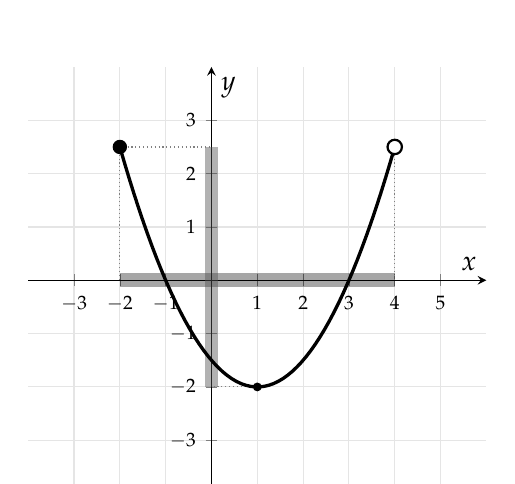
\begin{tikzpicture}
\begin{axis}[width=7.4cm,height=7cm,axis lines=middle,xmin=-4,xmax=6,ymin=-4,ymax=4,
  xtick={-3,-2,-1,1,2,3,4,5},ytick={-3,-2,-1,1,2,3},grid=major,grid style={gray!20},
  xlabel={$x$},ylabel={$y$},tick label style={font=\scriptsize}]
\draw[FangTeal,line width=5pt,opacity=0.35](axis cs:-2,0)--(axis cs:4,0);
\draw[FangGold,line width=5pt,opacity=0.45](axis cs:0,-2)--(axis cs:0,2.5);
\draw[densely dotted,gray](axis cs:-2,2.5)--(axis cs:-2,0);
\draw[densely dotted,gray](axis cs:4,2.5)--(axis cs:4,0);
\draw[densely dotted,gray](axis cs:-2,2.5)--(axis cs:0,2.5);
\draw[densely dotted,gray](axis cs:1,-2)--(axis cs:0,-2);
\addplot[FangBlue,very thick,domain=-2:4,samples=60]{0.5*(x-1)^2-2};
\fill[FangBlue](axis cs:-2,2.5) circle(2.6pt);
\draw[FangBlue,thick,fill=white](axis cs:4,2.5) circle(2.6pt);
\fill[FangBlue](axis cs:1,-2) circle(1.6pt);
\end{axis}
\end{tikzpicture}
\end{minipage}\hfill
\begin{minipage}[t]{0.47\textwidth}\vspace{4pt}
Shine a light from above: the graph's \textbf{shadow on the $x$-axis} (teal) is the \textbf{domain}. Shine it from the side: the \textbf{shadow on the $y$-axis} (gold) is the \textbf{range}.

\textbf{Read the domain} left to right: from $x=-2$ (closed dot, included) to $x=4$ (open dot, not included):
\[\text{Domain} = [-2,\,4).\]
\textbf{Read the range} bottom to top: the lowest point is the vertex, $y=-2$. The highest $y$ is $2.5$ — the open dot does \emph{not} reach it, but the closed dot at $(-2,\,2.5)$ does:
\[\text{Range} = [-2,\,2.5].\]
\end{minipage}

\begin{warn}
\textbf{Watch out:} an \textbf{arrow} means the graph keeps going, so that side goes to $\infty$ or $-\infty$. An open dot only leaves out that \emph{one point} — check whether another part of the graph reaches the same $y$.
\end{warn}

% ======================= PART 4 =======================
\sect{4}{From an equation: what could go wrong?}

\begin{idea}[Domain: start with all real numbers, then remove only what breaks]
\begin{tabular}{@{}lll@{}}
\textbf{1. Division by zero} & a denominator can't be $0$ & $\dfrac{1}{x-3}$: \ $x\neq3$\\[8pt]
\textbf{2. Even roots of negatives} & what is under $\sqrt{\ }$ must be $\ge0$ & $\sqrt{x+5}$: \ $x\ge-5$\\[4pt]
\textbf{3. Real-world limits} & time, length, people can't be negative & $t\ge0$, $n$ a whole number
\end{tabular}\par\smallskip
Nothing else breaks: polynomials, absolute value and \textbf{odd} roots like $\sqrt[3]{x}$ have domain $\R$.
\end{idea}

\textbf{Range: where can the outputs go?} Use the shape of the graph.

\begin{center}
\renewcommand{\arraystretch}{1.3}
\begin{tabular}{@{}lll@{}}
\toprule
\textbf{Function} & \textbf{Look at\ldots} & \textbf{Range}\\ \midrule
$a(x-h)^2+k$ & the vertex $(h,k)$: up if $a>0$, down if $a<0$ & $[k,\infty)$ or $(-\infty,k]$\\
$a\sqrt{x-h}+k$ & the starting point $(h,k)$ & $[k,\infty)$ if $a>0$, \ $(-\infty,k]$ if $a<0$\\
$a|x-h|+k$ & the vertex $(h,k)$ & $[k,\infty)$ or $(-\infty,k]$\\
$\dfrac{a}{x-h}+k$ & the horizontal asymptote $y=k$ & every $y$ except $k$\\
$mx+b$, \ $m\neq0$ & — & $\R$\\
\bottomrule
\end{tabular}
\end{center}

\begin{example}[Example 2 \;·\; a quadratic in standard form]
$f(x)=-x^2+6x-5$. \ Domain: a polynomial, so $\R$. \par
Vertex: $x=-\frac{b}{2a}=-\frac{6}{-2}=3$, and $f(3)=-9+18-5=4$. It opens down ($a<0$), so the highest output is $4$:
\quad Range $=(-\infty,\,4]$.
\end{example}

\begin{example}[Example 3 \;·\; a square root]
$g(x)=\sqrt{2x-6}+1$. \ Domain: $2x-6\ge0 \Rightarrow x\ge3$, so $[3,\infty)$.\par
Range: the square root starts at $0$ and grows, so $g$ starts at $0+1=1$ and grows: $[1,\infty)$. \ Simple case check: $g(3)=1$, $g(5)=3$. \checkmark
\end{example}

\begin{example}[Example 4 \;·\; a rational function — solve for $x$ to find the range]
$h(x)=\dfrac{2x+1}{x-4}$. \ Domain: $x\neq4$.\par
Range: set $y=\dfrac{2x+1}{x-4}$ and solve for $x$: \ $yx-4y=2x+1 \Rightarrow x(y-2)=4y+1 \Rightarrow x=\dfrac{4y+1}{y-2}$.\par
This works for every $y$ \textbf{except} $y=2$. So Range $=\{y\mid y\neq2\}$ — the horizontal asymptote.
\end{example}

\begin{warn}
\textbf{Common mistakes:} (1) Writing the domain of $\sqrt{x-4}$ as $x>4$ — it is $x\ge4$, because $\sqrt0=0$ is fine. \ (2) Saying the domain of $\frac{1}{x^2+1}$ excludes something — $x^2+1$ is never $0$, so the domain is $\R$. \ (3) Mixing up domain ($x$) and range ($y$).
\end{warn}

% ======================= PRACTICE =======================
\newpage
\sect{5}{Practice}
\ifkey\else\textit{Write every answer in interval notation (or as a list for sets of points). Test one or two easy numbers to check.}\fi

\medskip
\needspace{6cm}{\large\bfseries\color{FangBlue}A.\ Sets, tables and notation} \easy

\begin{enumerate}[leftmargin=*,label=\textbf{\arabic*.},itemsep=6pt]
\np[4cm]\item Find the domain and range: \ $\{(-2,3),\ (0,5),\ (1,3),\ (4,-1)\}$
\work[1.2cm]{Domain $\{-2,0,1,4\}$; \quad Range $\{-1,3,5\}$ (write $3$ only once).}

\np[4cm]\item Find the domain and range from the table. Is it a function?
\qquad\begin{tabular}{c|ccccc}$x$&$-3$&$-1$&$0$&$2$&$5$\\\hline $y$&$7$&$7$&$1$&$-2$&$0$\end{tabular}
\work[1.2cm]{Domain $\{-3,-1,0,2,5\}$; \quad Range $\{-2,0,1,7\}$. \quad Yes, a function: no $x$ repeats (a repeated $y$ is fine).}

\np[4cm]\item Write in interval notation: \quad (a) $-4\le x<1$ \qquad (b) $x>-2$ \qquad (c) $x\le0$ or $x>3$ \qquad (d) all reals except $-5$
\work[1.4cm]{(a) $[-4,1)$ \qquad (b) $(-2,\infty)$ \qquad (c) $(-\infty,0]\cup(3,\infty)$ \qquad (d) $(-\infty,-5)\cup(-5,\infty)$}
\end{enumerate}

\needspace{9cm}{\large\bfseries\color{FangBlue}B.\ From a graph} \medium

\textit{Give the domain and range of each graph. Arrows mean the graph continues.}

\begin{enumerate}[resume,leftmargin=*,label=\textbf{\arabic*.},itemsep=4pt]
\item[] \hspace*{-1.2em}\begin{tabular}{@{}c@{\hspace{4pt}}c@{\hspace{4pt}}c@{}}
\textbf{4.} \gr{\addplot[FangBlue,very thick] coordinates {(-3,-1)(4,3)}; \cls{-3}{-1}\opn{4}{3}} &
\textbf{5.} \gr{\addplot[FangBlue,very thick,domain=-1.8:3.8,samples=50,<->,>=Stealth]{(x-1)^2-4}; \cls{1}{-4}} &
\textbf{6.} \gr{\addplot[FangBlue,very thick,domain=-2:5.8,samples=80,->,>=Stealth]{sqrt(x+2)+1}; \cls{-2}{1}}\\[-2pt]
\ifkey{\small\color{FangGreen}$D=[-3,4)$, \ $R=[-1,3)$}\else{\small $D$ = \underline{\hspace{1.5cm}} \ $R$ = \underline{\hspace{1.5cm}}}\fi & \ifkey{\small\color{FangGreen}$D=\R$, \ $R=[-4,\infty)$}\else{\small $D$ = \underline{\hspace{1.5cm}} \ $R$ = \underline{\hspace{1.5cm}}}\fi & \ifkey{\small\color{FangGreen}$D=[-2,\infty)$, \ $R=[1,\infty)$}\else{\small $D$ = \underline{\hspace{1.5cm}} \ $R$ = \underline{\hspace{1.5cm}}}\fi\\[6pt]
\textbf{7.} \gr{\addplot[FangBlue,very thick,domain=-5.5:5.5,samples=111,<->,>=Stealth]{-abs(x)+3};} &
\textbf{8.} \gr{\addplot[gray,dashed] coordinates {(2,-6)(2,6)}; \addplot[gray,dashed] coordinates {(-6,1)(6,1)};
  \addplot[FangBlue,very thick,domain=-5.8:1.8,samples=80]{1/(x-2)+1}; \addplot[FangBlue,very thick,domain=2.2:5.8,samples=80]{1/(x-2)+1};} &
\textbf{9.} \gr{\addplot[FangBlue,very thick] coordinates {(-4,2)(-1,2)}; \addplot[FangBlue,very thick] coordinates {(-1,-2)(3,1)}; \cls{-4}{2}\opn{-1}{2}\cls{-1}{-2}\cls{3}{1}}\\[-2pt]
\ifkey{\small\color{FangGreen}$D=\R$, \ $R=(-\infty,3]$}\else{\small $D$ = \underline{\hspace{1.5cm}} \ $R$ = \underline{\hspace{1.5cm}}}\fi & \ifkey{\small\color{FangGreen}$D: x\neq2$, \ $R: y\neq1$ \ (asymptotes)}\else{\small $D$ = \underline{\hspace{1.5cm}} \ $R$ = \underline{\hspace{1.5cm}}}\fi & \ifkey{\small\color{FangGreen}$D=[-4,3]$, \ $R=[-2,1]\cup\{2\}$}\else{\small $D$ = \underline{\hspace{1.5cm}} \ $R$ = \underline{\hspace{1.5cm}}}\fi
\end{tabular}
\ifkey\else\vspace{1.2cm}\fi
\setcounter{enumi}{9}
\end{enumerate}
\ifkey{\small\textit{Note on 9:} the left piece is flat at $y=2$, so $2$ is in the range even though the open dot leaves out $(-1,2)$; the right piece covers $y$ from $-2$ to $1$.}\fi

\needspace{6cm}{\large\bfseries\color{FangBlue}C.\ Domain from an equation} \medium

\begin{multicols}{2}
\begin{enumerate}[resume,leftmargin=*,label=\textbf{\arabic*.},itemsep=4pt]
\setcounter{enumi}{9}
\item $f(x)=3x^2-5x+1$ \work[0.9cm]{$\R$ — a polynomial.}
\item $g(x)=\sqrt{x-6}$ \work[0.9cm]{$x-6\ge0$: \ $[6,\infty)$}
\item $h(x)=\sqrt{10-2x}$ \work[0.9cm]{$10-2x\ge0 \Rightarrow x\le5$: \ $(-\infty,5]$}
\item $k(x)=\dfrac{x+1}{x-7}$ \work[0.9cm]{$x\neq7$: \ $(-\infty,7)\cup(7,\infty)$}
\item $m(x)=\dfrac{5}{x^2-9}$ \work[0.9cm]{$x^2\neq9$, so $x\neq\pm3$: \ $(-\infty,-3)\cup(-3,3)\cup(3,\infty)$}
\item $p(x)=\sqrt[3]{x-4}$ \work[0.9cm]{$\R$ — odd roots accept negatives.}
\item $q(x)=\dfrac{\sqrt{x+2}}{x-3}$ \work[0.9cm]{Need $x\ge-2$ \textbf{and} $x\neq3$: \ $[-2,3)\cup(3,\infty)$}
\item $r(x)=\dfrac{4}{x^2+1}$ \work[0.9cm]{$x^2+1\ge1$, never $0$: \ $\R$}
\end{enumerate}
\end{multicols}

\needspace{6cm}{\large\bfseries\color{FangBlue}D.\ Domain and range from an equation} \medium\ \hard

\begin{enumerate}[resume,leftmargin=*,label=\textbf{\arabic*.},itemsep=6pt]
\setcounter{enumi}{17}
\np\item \medium\ $f(x)=(x-3)^2+2$
\work[1.6cm]{Domain $\R$. Vertex $(3,2)$, opens up: Range $[2,\infty)$.}
\np\item \medium\ $f(x)=-2x^2+8x-1$
\work[2cm]{Domain $\R$. Vertex at $x=-\frac{8}{2(-2)}=2$, \ $f(2)=-8+16-1=7$. Opens down: Range $(-\infty,7]$.}
\np\item \medium\ $f(x)=\sqrt{x+4}-3$
\work[1.6cm]{Domain: $x+4\ge0$, so $[-4,\infty)$. Starts at $(-4,-3)$ and rises: Range $[-3,\infty)$.}
\np\item \hard\ $f(x)=-\sqrt{9-x}+5$
\work[2cm]{Domain: $9-x\ge0 \Rightarrow x\le9$: $(-\infty,9]$. The root is $\ge0$, so $-\sqrt{\ }\le0$ and $f(x)\le5$: Range $(-\infty,5]$. \\ Check: $f(9)=5$, $f(0)=-3+5=2$.}
\np\item \medium\ $f(x)=|x+1|-4$
\work[1.6cm]{Domain $\R$. Vertex $(-1,-4)$, V opens up: Range $[-4,\infty)$.}
\np\item \medium\ $f(x)=\dfrac{2}{x+3}-1$
\work[1.6cm]{Domain $x\neq-3$. Horizontal asymptote $y=-1$ (the fraction $\frac{2}{x+3}$ is never $0$): Range $y\neq-1$, i.e.\ $(-\infty,-1)\cup(-1,\infty)$.}
\np\item \hard\ $f(x)=\dfrac{3x-1}{x+2}$ \quad (find the range by solving for $x$)
\work[2.4cm]{Domain $x\neq-2$. \ $y(x+2)=3x-1 \Rightarrow yx-3x=-1-2y \Rightarrow x(y-3)=-1-2y \Rightarrow x=\dfrac{-1-2y}{y-3}$. \\ Every $y$ works except $y=3$: Range $(-\infty,3)\cup(3,\infty)$.}
\end{enumerate}

\needspace{6cm}{\large\bfseries\color{FangBlue}E.\ Real-world domain and range} \medium

\begin{enumerate}[resume,leftmargin=*,label=\textbf{\arabic*.},itemsep=6pt]
\setcounter{enumi}{24}
\np\item Movie tickets cost \$12 each. A group of at most $8$ friends buys $n$ tickets, and the cost is $C(n)=12n$. Give a reasonable domain and range.
\work[1.8cm]{$n$ must be a whole number: Domain $\{0,1,2,\dots,8\}$. \ Range $\{0,12,24,\dots,96\}$. \\ (A list, not an interval — you can't buy $2.5$ tickets.)}
\np\item A ball is thrown upward. Its height in feet after $t$ seconds is $h(t)=-16t^2+64t$, until it hits the ground. Find the domain and range.
\work[2.6cm]{It hits the ground when $h(t)=0$: $-16t(t-4)=0$, so $t=0$ or $t=4$. \ Domain $[0,4]$. \\ Highest point at $t=-\frac{64}{2(-16)}=2$: $h(2)=-64+128=64$. \ Range $[0,64]$.}
\end{enumerate}

\needspace{6cm}{\large\bfseries\color{FangBlue}F.\ Challenge} \hard

\begin{enumerate}[resume,leftmargin=*,label=\textbf{\arabic*.},itemsep=6pt]
\setcounter{enumi}{26}
\np\item $f(x)=\sqrt{x^2-9}$
\work[2.2cm]{Need $x^2-9\ge0$, i.e.\ $x^2\ge9$: $x\le-3$ or $x\ge3$. \ Domain $(-\infty,-3]\cup[3,\infty)$. \\ $x^2-9$ takes every value $\ge0$, so Range $[0,\infty)$.}
\np\item $f(x)=\dfrac{x^2-4}{x-2}$
\work[2.2cm]{Domain $x\neq2$. For $x\neq2$, $f(x)=\dfrac{(x-2)(x+2)}{x-2}=x+2$ — a line with a \textbf{hole} at $(2,4)$. \\ So every $y$ except $4$: Range $(-\infty,4)\cup(4,\infty)$.}
\np\item $f(x)=\sqrt{16-x^2}$ \quad (Hint: what shape is the graph?)
\work[2.2cm]{Need $16-x^2\ge0$: Domain $[-4,4]$. The graph is the top half of the circle $x^2+y^2=16$, so it goes from $0$ up to $\sqrt{16}=4$: Range $[0,4]$.}
\end{enumerate}

\ifkey\else
\vfill
\begin{simple}
\textbf{Before you hand it in:} Did you use $[\ ]$ for included endpoints and $(\ )$ for $\infty$ and open dots? Did you test one easy number in each domain?
\end{simple}
\fi

\end{document}
"
% =====================================================================
\documentclass[11pt,letterpaper]{article}
\usepackage[margin=0.8in,top=0.85in,bottom=0.8in]{geometry}
\usepackage{mathpazo}
\usepackage[T1]{fontenc}
\usepackage{amsmath,amssymb}
\usepackage{xcolor}
\usepackage{enumitem}
\usepackage{multicol}
\usepackage{booktabs}
\usepackage{needspace}
\usepackage{fancyhdr}
\usepackage[most]{tcolorbox}
\usepackage{pgfplots}
\pgfplotsset{compat=1.17}
\usetikzlibrary{arrows.meta}

\definecolor{FangBlue}{HTML}{1F4E79}
\definecolor{FangTeal}{HTML}{0F7C7C}
\definecolor{FangGold}{HTML}{C9962B}
\definecolor{FangRed}{HTML}{B3261E}
\definecolor{FangGreen}{HTML}{2E8B57}
\definecolor{FangPurple}{HTML}{6A4BD8}
\definecolor{Soft}{HTML}{F4F7FB}
% black-and-white version: pdflatex with \def\isbw{1} before \input
\ifdefined\isbw
\definecolor{FangBlue}{HTML}{000000}\definecolor{FangTeal}{HTML}{000000}\definecolor{FangGold}{HTML}{555555}
\definecolor{FangRed}{HTML}{000000}\definecolor{FangGreen}{HTML}{000000}\definecolor{FangPurple}{HTML}{000000}\definecolor{Soft}{HTML}{FFFFFF}
\fi

\newif\ifkey
\ifdefined\iskey \keytrue \else \keyfalse \fi

\pagestyle{fancy}\fancyhf{}
\renewcommand{\headrulewidth}{0.4pt}
\fancyhead[L]{\small\color{FangBlue}\textbf{Prof. Fang Math} \,|\, Algebra 2 \,·\, 2-1 Domain \& Range}
\fancyhead[R]{\small\ifkey\textcolor{FangRed}{\textbf{ANSWER KEY}}\else Name: \underline{\hspace{4.2cm}}\fi}
\fancyfoot[C]{\small\thepage}
\fancyfoot[R]{\scriptsize\color{gray}fangmath.com}
\setlength{\headheight}{14pt}
\setlength{\parindent}{0pt}
\setlength{\parskip}{4pt}

% ---------- boxes ----------
\newtcolorbox{idea}[1][]{colback=Soft,colframe=FangBlue,boxrule=0.8pt,arc=3pt,left=8pt,right=8pt,top=6pt,bottom=6pt,
  fonttitle=\bfseries,coltitle=white,colbacktitle=FangBlue,title={#1}}
\newtcolorbox{example}[1][]{colback=white,colframe=FangTeal,boxrule=0.6pt,arc=3pt,left=8pt,right=8pt,top=5pt,bottom=5pt,
  fonttitle=\bfseries,coltitle=FangTeal,colbacktitle=white,title={#1},attach boxed title to top left={xshift=8pt,yshift=-7pt},boxed title style={boxrule=0pt,colframe=white}, enhanced}
\newtcolorbox{warn}{colback=FangRed!5,colframe=FangRed,boxrule=0.6pt,arc=3pt,left=8pt,right=8pt,top=4pt,bottom=4pt,leftrule=3pt}
\newtcolorbox{simple}{colback=FangGold!10,colframe=FangGold,boxrule=0.6pt,arc=3pt,left=8pt,right=8pt,top=4pt,bottom=4pt,leftrule=3pt}
\newtcolorbox{sol}{colback=FangGreen!6,colframe=FangGreen,boxrule=0.5pt,arc=2pt,left=6pt,right=6pt,top=3pt,bottom=3pt,breakable}

\newcommand{\badge}[2]{\tcbox[on line,colback=#1,colframe=#1,coltext=white,boxrule=0pt,arc=6pt,left=4pt,right=4pt,top=1pt,bottom=1pt,fontupper=\scriptsize\bfseries]{#2}}
\newcommand{\easy}{\badge{FangGreen}{EASY}}
\newcommand{\medium}{\badge{FangTeal}{MEDIUM}}
\newcommand{\hard}{\badge{FangRed}{HARD}}
\newcommand{\work}[2][]{\ifkey\begin{sol}#2\end{sol}\else\vspace*{#1}\fi}
\newcommand{\np}[1][6cm]{\needspace{#1}}
\newcommand{\sect}[2]{\par\needspace{7cm}\medskip{\Large\bfseries\color{FangBlue}\tcbox[on line,colback=FangBlue,colframe=FangBlue,coltext=white,arc=2pt,boxrule=0pt,left=5pt,right=5pt,top=1pt,bottom=1pt]{#1}\ #2}\par\smallskip}


\newcommand{\R}{\mathbb{R}}
% small graph for practice problems: \gr{plot commands}
\newcommand{\gr}[2][]{\begin{tikzpicture}\begin{axis}[width=5.0cm,height=5.0cm,axis lines=middle,xmin=-6,xmax=6,ymin=-6,ymax=6,
  xtick={-4,-2,2,4},ytick={-4,-2,2,4},grid=both,minor tick num=1,grid style={gray!18},major grid style={gray!30},
  xlabel={\scriptsize$x$},ylabel={\scriptsize$y$},tick label style={font=\tiny},clip=true,#1]#2\end{axis}\end{tikzpicture}}
\newcommand{\opn}[2]{\draw[FangBlue,thick,fill=white](axis cs:#1,#2) circle(2.4pt);}
\newcommand{\cls}[2]{\fill[FangBlue](axis cs:#1,#2) circle(2.4pt);}

\begin{document}

% ======================= TITLE =======================
\begin{center}
{\color{FangBlue}\Huge\bfseries Domain \& Range}\\[2pt]
{\large What can go in? What can come out?}
\ifkey\\[3pt]{\color{FangRed}\large\bfseries Answer Key with complete solutions}\fi
\end{center}
\vspace{-4pt}

\begin{idea}[The big idea]
A function is a machine: you put in an $x$, it gives back one $y$.
\begin{itemize}[leftmargin=*,itemsep=1pt,topsep=2pt]
\item The \textbf{domain} is every $x$ you are \textbf{allowed to put in}. \quad (inputs, the horizontal direction)
\item The \textbf{range} is every $y$ that can \textbf{actually come out}. \quad (outputs, the vertical direction)
\end{itemize}
\end{idea}

\begin{simple}
\textbf{Simple case first.} For $f(x)=\sqrt{x}$, try a few inputs: $f(9)=3$, $f(0)=0$, but $f(-4)$ is not a real number. So the domain is $x\ge0$. And since a square root is never negative, the outputs are $y\ge0$. Testing a few easy numbers is always a good way to start.
\end{simple}

% ======================= PART 1 =======================
\sect{1}{Three ways to write a set of numbers}

\begin{center}
\renewcommand{\arraystretch}{1.35}
\begin{tabular}{@{}llll@{}}
\toprule
\textbf{In words} & \textbf{Inequality} & \textbf{Interval notation} & \textbf{Set-builder}\\ \midrule
from $-2$ to $5$, including $-2$, not $5$ & $-2\le x<5$ & $[-2,\,5)$ & $\{x\mid -2\le x<5\}$\\
greater than $3$ & $x>3$ & $(3,\,\infty)$ & $\{x\mid x>3\}$\\
at most $-1$ & $x\le -1$ & $(-\infty,\,-1]$ & $\{x\mid x\le-1\}$\\
all real numbers & — & $(-\infty,\,\infty)$ & $\R$\\
every number except $2$ & $x\neq2$ & $(-\infty,2)\cup(2,\infty)$ & $\{x\mid x\neq 2\}$\\
\bottomrule
\end{tabular}
\end{center}

\begin{multicols}{2}
\textbf{Square bracket} $[\ ]$: the endpoint is \textbf{included} (closed dot $\bullet$, $\le$ or $\ge$).\par
\textbf{Parenthesis} $(\ )$: the endpoint is \textbf{not included} (open dot $\circ$, $<$ or $>$).
\columnbreak

$\infty$ is not a number you can reach, so it \textbf{always} gets a parenthesis.\par
$\cup$ means ``or'' — it joins two pieces.
\end{multicols}

% ======================= PART 2 =======================
\sect{2}{From points, a table, or a mapping}

\begin{example}[Example 1]
$\{(-1,4),\ (0,2),\ (3,4),\ (5,-1)\}$ \qquad Domain: list the $x$'s: $\{-1,0,3,5\}$. \quad Range: list the $y$'s: $\{-1,2,4\}$.\par
List each value \textbf{once}, from smallest to largest ($4$ appears twice but is written once).
\end{example}

% ======================= PART 3 =======================
\sect{3}{From a graph: look at the shadows}

\begin{minipage}[t]{0.5\textwidth}\vspace{0pt}\centering
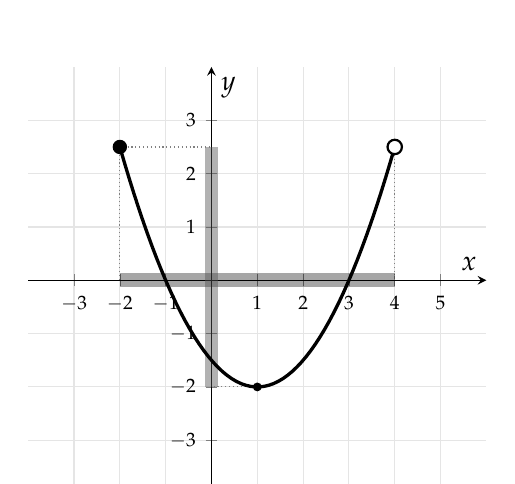
\begin{tikzpicture}
\begin{axis}[width=7.4cm,height=7cm,axis lines=middle,xmin=-4,xmax=6,ymin=-4,ymax=4,
  xtick={-3,-2,-1,1,2,3,4,5},ytick={-3,-2,-1,1,2,3},grid=major,grid style={gray!20},
  xlabel={$x$},ylabel={$y$},tick label style={font=\scriptsize}]
\draw[FangTeal,line width=5pt,opacity=0.35](axis cs:-2,0)--(axis cs:4,0);
\draw[FangGold,line width=5pt,opacity=0.45](axis cs:0,-2)--(axis cs:0,2.5);
\draw[densely dotted,gray](axis cs:-2,2.5)--(axis cs:-2,0);
\draw[densely dotted,gray](axis cs:4,2.5)--(axis cs:4,0);
\draw[densely dotted,gray](axis cs:-2,2.5)--(axis cs:0,2.5);
\draw[densely dotted,gray](axis cs:1,-2)--(axis cs:0,-2);
\addplot[FangBlue,very thick,domain=-2:4,samples=60]{0.5*(x-1)^2-2};
\fill[FangBlue](axis cs:-2,2.5) circle(2.6pt);
\draw[FangBlue,thick,fill=white](axis cs:4,2.5) circle(2.6pt);
\fill[FangBlue](axis cs:1,-2) circle(1.6pt);
\end{axis}
\end{tikzpicture}
\end{minipage}\hfill
\begin{minipage}[t]{0.47\textwidth}\vspace{4pt}
Shine a light from above: the graph's \textbf{shadow on the $x$-axis} (teal) is the \textbf{domain}. Shine it from the side: the \textbf{shadow on the $y$-axis} (gold) is the \textbf{range}.

\textbf{Read the domain} left to right: from $x=-2$ (closed dot, included) to $x=4$ (open dot, not included):
\[\text{Domain} = [-2,\,4).\]
\textbf{Read the range} bottom to top: the lowest point is the vertex, $y=-2$. The highest $y$ is $2.5$ — the open dot does \emph{not} reach it, but the closed dot at $(-2,\,2.5)$ does:
\[\text{Range} = [-2,\,2.5].\]
\end{minipage}

\begin{warn}
\textbf{Watch out:} an \textbf{arrow} means the graph keeps going, so that side goes to $\infty$ or $-\infty$. An open dot only leaves out that \emph{one point} — check whether another part of the graph reaches the same $y$.
\end{warn}

% ======================= PART 4 =======================
\sect{4}{From an equation: what could go wrong?}

\begin{idea}[Domain: start with all real numbers, then remove only what breaks]
\begin{tabular}{@{}lll@{}}
\textbf{1. Division by zero} & a denominator can't be $0$ & $\dfrac{1}{x-3}$: \ $x\neq3$\\[8pt]
\textbf{2. Even roots of negatives} & what is under $\sqrt{\ }$ must be $\ge0$ & $\sqrt{x+5}$: \ $x\ge-5$\\[4pt]
\textbf{3. Real-world limits} & time, length, people can't be negative & $t\ge0$, $n$ a whole number
\end{tabular}\par\smallskip
Nothing else breaks: polynomials, absolute value and \textbf{odd} roots like $\sqrt[3]{x}$ have domain $\R$.
\end{idea}

\textbf{Range: where can the outputs go?} Use the shape of the graph.

\begin{center}
\renewcommand{\arraystretch}{1.3}
\begin{tabular}{@{}lll@{}}
\toprule
\textbf{Function} & \textbf{Look at\ldots} & \textbf{Range}\\ \midrule
$a(x-h)^2+k$ & the vertex $(h,k)$: up if $a>0$, down if $a<0$ & $[k,\infty)$ or $(-\infty,k]$\\
$a\sqrt{x-h}+k$ & the starting point $(h,k)$ & $[k,\infty)$ if $a>0$, \ $(-\infty,k]$ if $a<0$\\
$a|x-h|+k$ & the vertex $(h,k)$ & $[k,\infty)$ or $(-\infty,k]$\\
$\dfrac{a}{x-h}+k$ & the horizontal asymptote $y=k$ & every $y$ except $k$\\
$mx+b$, \ $m\neq0$ & — & $\R$\\
\bottomrule
\end{tabular}
\end{center}

\begin{example}[Example 2 \;·\; a quadratic in standard form]
$f(x)=-x^2+6x-5$. \ Domain: a polynomial, so $\R$. \par
Vertex: $x=-\frac{b}{2a}=-\frac{6}{-2}=3$, and $f(3)=-9+18-5=4$. It opens down ($a<0$), so the highest output is $4$:
\quad Range $=(-\infty,\,4]$.
\end{example}

\begin{example}[Example 3 \;·\; a square root]
$g(x)=\sqrt{2x-6}+1$. \ Domain: $2x-6\ge0 \Rightarrow x\ge3$, so $[3,\infty)$.\par
Range: the square root starts at $0$ and grows, so $g$ starts at $0+1=1$ and grows: $[1,\infty)$. \ Simple case check: $g(3)=1$, $g(5)=3$. \checkmark
\end{example}

\begin{example}[Example 4 \;·\; a rational function — solve for $x$ to find the range]
$h(x)=\dfrac{2x+1}{x-4}$. \ Domain: $x\neq4$.\par
Range: set $y=\dfrac{2x+1}{x-4}$ and solve for $x$: \ $yx-4y=2x+1 \Rightarrow x(y-2)=4y+1 \Rightarrow x=\dfrac{4y+1}{y-2}$.\par
This works for every $y$ \textbf{except} $y=2$. So Range $=\{y\mid y\neq2\}$ — the horizontal asymptote.
\end{example}

\begin{warn}
\textbf{Common mistakes:} (1) Writing the domain of $\sqrt{x-4}$ as $x>4$ — it is $x\ge4$, because $\sqrt0=0$ is fine. \ (2) Saying the domain of $\frac{1}{x^2+1}$ excludes something — $x^2+1$ is never $0$, so the domain is $\R$. \ (3) Mixing up domain ($x$) and range ($y$).
\end{warn}

% ======================= PRACTICE =======================
\newpage
\sect{5}{Practice}
\ifkey\else\textit{Write every answer in interval notation (or as a list for sets of points). Test one or two easy numbers to check.}\fi

\medskip
\needspace{6cm}{\large\bfseries\color{FangBlue}A.\ Sets, tables and notation} \easy

\begin{enumerate}[leftmargin=*,label=\textbf{\arabic*.},itemsep=6pt]
\np[4cm]\item Find the domain and range: \ $\{(-2,3),\ (0,5),\ (1,3),\ (4,-1)\}$
\work[1.2cm]{Domain $\{-2,0,1,4\}$; \quad Range $\{-1,3,5\}$ (write $3$ only once).}

\np[4cm]\item Find the domain and range from the table. Is it a function?
\qquad\begin{tabular}{c|ccccc}$x$&$-3$&$-1$&$0$&$2$&$5$\\\hline $y$&$7$&$7$&$1$&$-2$&$0$\end{tabular}
\work[1.2cm]{Domain $\{-3,-1,0,2,5\}$; \quad Range $\{-2,0,1,7\}$. \quad Yes, a function: no $x$ repeats (a repeated $y$ is fine).}

\np[4cm]\item Write in interval notation: \quad (a) $-4\le x<1$ \qquad (b) $x>-2$ \qquad (c) $x\le0$ or $x>3$ \qquad (d) all reals except $-5$
\work[1.4cm]{(a) $[-4,1)$ \qquad (b) $(-2,\infty)$ \qquad (c) $(-\infty,0]\cup(3,\infty)$ \qquad (d) $(-\infty,-5)\cup(-5,\infty)$}
\end{enumerate}

\needspace{9cm}{\large\bfseries\color{FangBlue}B.\ From a graph} \medium

\textit{Give the domain and range of each graph. Arrows mean the graph continues.}

\begin{enumerate}[resume,leftmargin=*,label=\textbf{\arabic*.},itemsep=4pt]
\item[] \hspace*{-1.2em}\begin{tabular}{@{}c@{\hspace{4pt}}c@{\hspace{4pt}}c@{}}
\textbf{4.} \gr{\addplot[FangBlue,very thick] coordinates {(-3,-1)(4,3)}; \cls{-3}{-1}\opn{4}{3}} &
\textbf{5.} \gr{\addplot[FangBlue,very thick,domain=-1.8:3.8,samples=50,<->,>=Stealth]{(x-1)^2-4}; \cls{1}{-4}} &
\textbf{6.} \gr{\addplot[FangBlue,very thick,domain=-2:5.8,samples=80,->,>=Stealth]{sqrt(x+2)+1}; \cls{-2}{1}}\\[-2pt]
\ifkey{\small\color{FangGreen}$D=[-3,4)$, \ $R=[-1,3)$}\else{\small $D$ = \underline{\hspace{1.5cm}} \ $R$ = \underline{\hspace{1.5cm}}}\fi & \ifkey{\small\color{FangGreen}$D=\R$, \ $R=[-4,\infty)$}\else{\small $D$ = \underline{\hspace{1.5cm}} \ $R$ = \underline{\hspace{1.5cm}}}\fi & \ifkey{\small\color{FangGreen}$D=[-2,\infty)$, \ $R=[1,\infty)$}\else{\small $D$ = \underline{\hspace{1.5cm}} \ $R$ = \underline{\hspace{1.5cm}}}\fi\\[6pt]
\textbf{7.} \gr{\addplot[FangBlue,very thick,domain=-5.5:5.5,samples=111,<->,>=Stealth]{-abs(x)+3};} &
\textbf{8.} \gr{\addplot[gray,dashed] coordinates {(2,-6)(2,6)}; \addplot[gray,dashed] coordinates {(-6,1)(6,1)};
  \addplot[FangBlue,very thick,domain=-5.8:1.8,samples=80]{1/(x-2)+1}; \addplot[FangBlue,very thick,domain=2.2:5.8,samples=80]{1/(x-2)+1};} &
\textbf{9.} \gr{\addplot[FangBlue,very thick] coordinates {(-4,2)(-1,2)}; \addplot[FangBlue,very thick] coordinates {(-1,-2)(3,1)}; \cls{-4}{2}\opn{-1}{2}\cls{-1}{-2}\cls{3}{1}}\\[-2pt]
\ifkey{\small\color{FangGreen}$D=\R$, \ $R=(-\infty,3]$}\else{\small $D$ = \underline{\hspace{1.5cm}} \ $R$ = \underline{\hspace{1.5cm}}}\fi & \ifkey{\small\color{FangGreen}$D: x\neq2$, \ $R: y\neq1$ \ (asymptotes)}\else{\small $D$ = \underline{\hspace{1.5cm}} \ $R$ = \underline{\hspace{1.5cm}}}\fi & \ifkey{\small\color{FangGreen}$D=[-4,3]$, \ $R=[-2,1]\cup\{2\}$}\else{\small $D$ = \underline{\hspace{1.5cm}} \ $R$ = \underline{\hspace{1.5cm}}}\fi
\end{tabular}
\ifkey\else\vspace{1.2cm}\fi
\setcounter{enumi}{9}
\end{enumerate}
\ifkey{\small\textit{Note on 9:} the left piece is flat at $y=2$, so $2$ is in the range even though the open dot leaves out $(-1,2)$; the right piece covers $y$ from $-2$ to $1$.}\fi

\needspace{6cm}{\large\bfseries\color{FangBlue}C.\ Domain from an equation} \medium

\begin{multicols}{2}
\begin{enumerate}[resume,leftmargin=*,label=\textbf{\arabic*.},itemsep=4pt]
\setcounter{enumi}{9}
\item $f(x)=3x^2-5x+1$ \work[0.9cm]{$\R$ — a polynomial.}
\item $g(x)=\sqrt{x-6}$ \work[0.9cm]{$x-6\ge0$: \ $[6,\infty)$}
\item $h(x)=\sqrt{10-2x}$ \work[0.9cm]{$10-2x\ge0 \Rightarrow x\le5$: \ $(-\infty,5]$}
\item $k(x)=\dfrac{x+1}{x-7}$ \work[0.9cm]{$x\neq7$: \ $(-\infty,7)\cup(7,\infty)$}
\item $m(x)=\dfrac{5}{x^2-9}$ \work[0.9cm]{$x^2\neq9$, so $x\neq\pm3$: \ $(-\infty,-3)\cup(-3,3)\cup(3,\infty)$}
\item $p(x)=\sqrt[3]{x-4}$ \work[0.9cm]{$\R$ — odd roots accept negatives.}
\item $q(x)=\dfrac{\sqrt{x+2}}{x-3}$ \work[0.9cm]{Need $x\ge-2$ \textbf{and} $x\neq3$: \ $[-2,3)\cup(3,\infty)$}
\item $r(x)=\dfrac{4}{x^2+1}$ \work[0.9cm]{$x^2+1\ge1$, never $0$: \ $\R$}
\end{enumerate}
\end{multicols}

\needspace{6cm}{\large\bfseries\color{FangBlue}D.\ Domain and range from an equation} \medium\ \hard

\begin{enumerate}[resume,leftmargin=*,label=\textbf{\arabic*.},itemsep=6pt]
\setcounter{enumi}{17}
\np\item \medium\ $f(x)=(x-3)^2+2$
\work[1.6cm]{Domain $\R$. Vertex $(3,2)$, opens up: Range $[2,\infty)$.}
\np\item \medium\ $f(x)=-2x^2+8x-1$
\work[2cm]{Domain $\R$. Vertex at $x=-\frac{8}{2(-2)}=2$, \ $f(2)=-8+16-1=7$. Opens down: Range $(-\infty,7]$.}
\np\item \medium\ $f(x)=\sqrt{x+4}-3$
\work[1.6cm]{Domain: $x+4\ge0$, so $[-4,\infty)$. Starts at $(-4,-3)$ and rises: Range $[-3,\infty)$.}
\np\item \hard\ $f(x)=-\sqrt{9-x}+5$
\work[2cm]{Domain: $9-x\ge0 \Rightarrow x\le9$: $(-\infty,9]$. The root is $\ge0$, so $-\sqrt{\ }\le0$ and $f(x)\le5$: Range $(-\infty,5]$. \\ Check: $f(9)=5$, $f(0)=-3+5=2$.}
\np\item \medium\ $f(x)=|x+1|-4$
\work[1.6cm]{Domain $\R$. Vertex $(-1,-4)$, V opens up: Range $[-4,\infty)$.}
\np\item \medium\ $f(x)=\dfrac{2}{x+3}-1$
\work[1.6cm]{Domain $x\neq-3$. Horizontal asymptote $y=-1$ (the fraction $\frac{2}{x+3}$ is never $0$): Range $y\neq-1$, i.e.\ $(-\infty,-1)\cup(-1,\infty)$.}
\np\item \hard\ $f(x)=\dfrac{3x-1}{x+2}$ \quad (find the range by solving for $x$)
\work[2.4cm]{Domain $x\neq-2$. \ $y(x+2)=3x-1 \Rightarrow yx-3x=-1-2y \Rightarrow x(y-3)=-1-2y \Rightarrow x=\dfrac{-1-2y}{y-3}$. \\ Every $y$ works except $y=3$: Range $(-\infty,3)\cup(3,\infty)$.}
\end{enumerate}

\needspace{6cm}{\large\bfseries\color{FangBlue}E.\ Real-world domain and range} \medium

\begin{enumerate}[resume,leftmargin=*,label=\textbf{\arabic*.},itemsep=6pt]
\setcounter{enumi}{24}
\np\item Movie tickets cost \$12 each. A group of at most $8$ friends buys $n$ tickets, and the cost is $C(n)=12n$. Give a reasonable domain and range.
\work[1.8cm]{$n$ must be a whole number: Domain $\{0,1,2,\dots,8\}$. \ Range $\{0,12,24,\dots,96\}$. \\ (A list, not an interval — you can't buy $2.5$ tickets.)}
\np\item A ball is thrown upward. Its height in feet after $t$ seconds is $h(t)=-16t^2+64t$, until it hits the ground. Find the domain and range.
\work[2.6cm]{It hits the ground when $h(t)=0$: $-16t(t-4)=0$, so $t=0$ or $t=4$. \ Domain $[0,4]$. \\ Highest point at $t=-\frac{64}{2(-16)}=2$: $h(2)=-64+128=64$. \ Range $[0,64]$.}
\end{enumerate}

\needspace{6cm}{\large\bfseries\color{FangBlue}F.\ Challenge} \hard

\begin{enumerate}[resume,leftmargin=*,label=\textbf{\arabic*.},itemsep=6pt]
\setcounter{enumi}{26}
\np\item $f(x)=\sqrt{x^2-9}$
\work[2.2cm]{Need $x^2-9\ge0$, i.e.\ $x^2\ge9$: $x\le-3$ or $x\ge3$. \ Domain $(-\infty,-3]\cup[3,\infty)$. \\ $x^2-9$ takes every value $\ge0$, so Range $[0,\infty)$.}
\np\item $f(x)=\dfrac{x^2-4}{x-2}$
\work[2.2cm]{Domain $x\neq2$. For $x\neq2$, $f(x)=\dfrac{(x-2)(x+2)}{x-2}=x+2$ — a line with a \textbf{hole} at $(2,4)$. \\ So every $y$ except $4$: Range $(-\infty,4)\cup(4,\infty)$.}
\np\item $f(x)=\sqrt{16-x^2}$ \quad (Hint: what shape is the graph?)
\work[2.2cm]{Need $16-x^2\ge0$: Domain $[-4,4]$. The graph is the top half of the circle $x^2+y^2=16$, so it goes from $0$ up to $\sqrt{16}=4$: Range $[0,4]$.}
\end{enumerate}

\ifkey\else
\vfill
\begin{simple}
\textbf{Before you hand it in:} Did you use $[\ ]$ for included endpoints and $(\ )$ for $\infty$ and open dots? Did you test one easy number in each domain?
\end{simple}
\fi

\end{document}
"
% =====================================================================
\documentclass[11pt,letterpaper]{article}
\usepackage[margin=0.8in,top=0.85in,bottom=0.8in]{geometry}
\usepackage{mathpazo}
\usepackage[T1]{fontenc}
\usepackage{amsmath,amssymb}
\usepackage{xcolor}
\usepackage{enumitem}
\usepackage{multicol}
\usepackage{booktabs}
\usepackage{needspace}
\usepackage{fancyhdr}
\usepackage[most]{tcolorbox}
\usepackage{pgfplots}
\pgfplotsset{compat=1.17}
\usetikzlibrary{arrows.meta}

\definecolor{FangBlue}{HTML}{1F4E79}
\definecolor{FangTeal}{HTML}{0F7C7C}
\definecolor{FangGold}{HTML}{C9962B}
\definecolor{FangRed}{HTML}{B3261E}
\definecolor{FangGreen}{HTML}{2E8B57}
\definecolor{FangPurple}{HTML}{6A4BD8}
\definecolor{Soft}{HTML}{F4F7FB}
% black-and-white version: pdflatex with \def\isbw{1} before \input
\ifdefined\isbw
\definecolor{FangBlue}{HTML}{000000}\definecolor{FangTeal}{HTML}{000000}\definecolor{FangGold}{HTML}{555555}
\definecolor{FangRed}{HTML}{000000}\definecolor{FangGreen}{HTML}{000000}\definecolor{FangPurple}{HTML}{000000}\definecolor{Soft}{HTML}{FFFFFF}
\fi

\newif\ifkey
\ifdefined\iskey \keytrue \else \keyfalse \fi

\pagestyle{fancy}\fancyhf{}
\renewcommand{\headrulewidth}{0.4pt}
\fancyhead[L]{\small\color{FangBlue}\textbf{Prof. Fang Math} \,|\, Algebra 2 \,·\, 2-1 Domain \& Range}
\fancyhead[R]{\small\ifkey\textcolor{FangRed}{\textbf{ANSWER KEY}}\else Name: \underline{\hspace{4.2cm}}\fi}
\fancyfoot[C]{\small\thepage}
\fancyfoot[R]{\scriptsize\color{gray}fangmath.com}
\setlength{\headheight}{14pt}
\setlength{\parindent}{0pt}
\setlength{\parskip}{4pt}

% ---------- boxes ----------
\newtcolorbox{idea}[1][]{colback=Soft,colframe=FangBlue,boxrule=0.8pt,arc=3pt,left=8pt,right=8pt,top=6pt,bottom=6pt,
  fonttitle=\bfseries,coltitle=white,colbacktitle=FangBlue,title={#1}}
\newtcolorbox{example}[1][]{colback=white,colframe=FangTeal,boxrule=0.6pt,arc=3pt,left=8pt,right=8pt,top=5pt,bottom=5pt,
  fonttitle=\bfseries,coltitle=FangTeal,colbacktitle=white,title={#1},attach boxed title to top left={xshift=8pt,yshift=-7pt},boxed title style={boxrule=0pt,colframe=white}, enhanced}
\newtcolorbox{warn}{colback=FangRed!5,colframe=FangRed,boxrule=0.6pt,arc=3pt,left=8pt,right=8pt,top=4pt,bottom=4pt,leftrule=3pt}
\newtcolorbox{simple}{colback=FangGold!10,colframe=FangGold,boxrule=0.6pt,arc=3pt,left=8pt,right=8pt,top=4pt,bottom=4pt,leftrule=3pt}
\newtcolorbox{sol}{colback=FangGreen!6,colframe=FangGreen,boxrule=0.5pt,arc=2pt,left=6pt,right=6pt,top=3pt,bottom=3pt,breakable}

\newcommand{\badge}[2]{\tcbox[on line,colback=#1,colframe=#1,coltext=white,boxrule=0pt,arc=6pt,left=4pt,right=4pt,top=1pt,bottom=1pt,fontupper=\scriptsize\bfseries]{#2}}
\newcommand{\easy}{\badge{FangGreen}{EASY}}
\newcommand{\medium}{\badge{FangTeal}{MEDIUM}}
\newcommand{\hard}{\badge{FangRed}{HARD}}
\newcommand{\work}[2][]{\ifkey\begin{sol}#2\end{sol}\else\vspace*{#1}\fi}
\newcommand{\np}[1][6cm]{\needspace{#1}}
\newcommand{\sect}[2]{\par\needspace{7cm}\medskip{\Large\bfseries\color{FangBlue}\tcbox[on line,colback=FangBlue,colframe=FangBlue,coltext=white,arc=2pt,boxrule=0pt,left=5pt,right=5pt,top=1pt,bottom=1pt]{#1}\ #2}\par\smallskip}


\newcommand{\R}{\mathbb{R}}
% small graph for practice problems: \gr{plot commands}
\newcommand{\gr}[2][]{\begin{tikzpicture}\begin{axis}[width=5.0cm,height=5.0cm,axis lines=middle,xmin=-6,xmax=6,ymin=-6,ymax=6,
  xtick={-4,-2,2,4},ytick={-4,-2,2,4},grid=both,minor tick num=1,grid style={gray!18},major grid style={gray!30},
  xlabel={\scriptsize$x$},ylabel={\scriptsize$y$},tick label style={font=\tiny},clip=true,#1]#2\end{axis}\end{tikzpicture}}
\newcommand{\opn}[2]{\draw[FangBlue,thick,fill=white](axis cs:#1,#2) circle(2.4pt);}
\newcommand{\cls}[2]{\fill[FangBlue](axis cs:#1,#2) circle(2.4pt);}

\begin{document}

% ======================= TITLE =======================
\begin{center}
{\color{FangBlue}\Huge\bfseries Domain \& Range}\\[2pt]
{\large What can go in? What can come out?}
\ifkey\\[3pt]{\color{FangRed}\large\bfseries Answer Key with complete solutions}\fi
\end{center}
\vspace{-4pt}

\begin{idea}[The big idea]
A function is a machine: you put in an $x$, it gives back one $y$.
\begin{itemize}[leftmargin=*,itemsep=1pt,topsep=2pt]
\item The \textbf{domain} is every $x$ you are \textbf{allowed to put in}. \quad (inputs, the horizontal direction)
\item The \textbf{range} is every $y$ that can \textbf{actually come out}. \quad (outputs, the vertical direction)
\end{itemize}
\end{idea}

\begin{simple}
\textbf{Simple case first.} For $f(x)=\sqrt{x}$, try a few inputs: $f(9)=3$, $f(0)=0$, but $f(-4)$ is not a real number. So the domain is $x\ge0$. And since a square root is never negative, the outputs are $y\ge0$. Testing a few easy numbers is always a good way to start.
\end{simple}

% ======================= PART 1 =======================
\sect{1}{Three ways to write a set of numbers}

\begin{center}
\renewcommand{\arraystretch}{1.35}
\begin{tabular}{@{}llll@{}}
\toprule
\textbf{In words} & \textbf{Inequality} & \textbf{Interval notation} & \textbf{Set-builder}\\ \midrule
from $-2$ to $5$, including $-2$, not $5$ & $-2\le x<5$ & $[-2,\,5)$ & $\{x\mid -2\le x<5\}$\\
greater than $3$ & $x>3$ & $(3,\,\infty)$ & $\{x\mid x>3\}$\\
at most $-1$ & $x\le -1$ & $(-\infty,\,-1]$ & $\{x\mid x\le-1\}$\\
all real numbers & — & $(-\infty,\,\infty)$ & $\R$\\
every number except $2$ & $x\neq2$ & $(-\infty,2)\cup(2,\infty)$ & $\{x\mid x\neq 2\}$\\
\bottomrule
\end{tabular}
\end{center}

\begin{multicols}{2}
\textbf{Square bracket} $[\ ]$: the endpoint is \textbf{included} (closed dot $\bullet$, $\le$ or $\ge$).\par
\textbf{Parenthesis} $(\ )$: the endpoint is \textbf{not included} (open dot $\circ$, $<$ or $>$).
\columnbreak

$\infty$ is not a number you can reach, so it \textbf{always} gets a parenthesis.\par
$\cup$ means ``or'' — it joins two pieces.
\end{multicols}

% ======================= PART 2 =======================
\sect{2}{From points, a table, or a mapping}

\begin{example}[Example 1]
$\{(-1,4),\ (0,2),\ (3,4),\ (5,-1)\}$ \qquad Domain: list the $x$'s: $\{-1,0,3,5\}$. \quad Range: list the $y$'s: $\{-1,2,4\}$.\par
List each value \textbf{once}, from smallest to largest ($4$ appears twice but is written once).
\end{example}

% ======================= PART 3 =======================
\sect{3}{From a graph: look at the shadows}

\begin{minipage}[t]{0.5\textwidth}\vspace{0pt}\centering
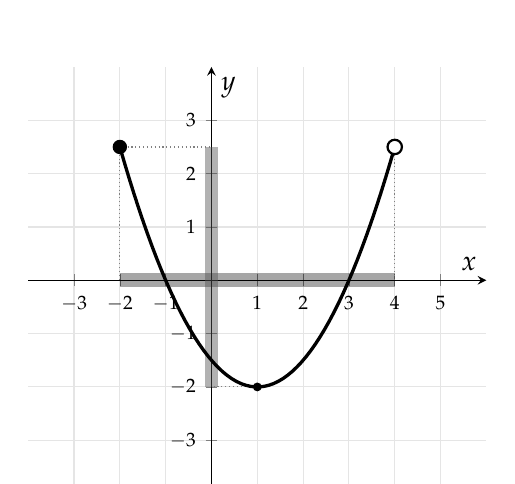
\begin{tikzpicture}
\begin{axis}[width=7.4cm,height=7cm,axis lines=middle,xmin=-4,xmax=6,ymin=-4,ymax=4,
  xtick={-3,-2,-1,1,2,3,4,5},ytick={-3,-2,-1,1,2,3},grid=major,grid style={gray!20},
  xlabel={$x$},ylabel={$y$},tick label style={font=\scriptsize}]
\draw[FangTeal,line width=5pt,opacity=0.35](axis cs:-2,0)--(axis cs:4,0);
\draw[FangGold,line width=5pt,opacity=0.45](axis cs:0,-2)--(axis cs:0,2.5);
\draw[densely dotted,gray](axis cs:-2,2.5)--(axis cs:-2,0);
\draw[densely dotted,gray](axis cs:4,2.5)--(axis cs:4,0);
\draw[densely dotted,gray](axis cs:-2,2.5)--(axis cs:0,2.5);
\draw[densely dotted,gray](axis cs:1,-2)--(axis cs:0,-2);
\addplot[FangBlue,very thick,domain=-2:4,samples=60]{0.5*(x-1)^2-2};
\fill[FangBlue](axis cs:-2,2.5) circle(2.6pt);
\draw[FangBlue,thick,fill=white](axis cs:4,2.5) circle(2.6pt);
\fill[FangBlue](axis cs:1,-2) circle(1.6pt);
\end{axis}
\end{tikzpicture}
\end{minipage}\hfill
\begin{minipage}[t]{0.47\textwidth}\vspace{4pt}
Shine a light from above: the graph's \textbf{shadow on the $x$-axis} (teal) is the \textbf{domain}. Shine it from the side: the \textbf{shadow on the $y$-axis} (gold) is the \textbf{range}.

\textbf{Read the domain} left to right: from $x=-2$ (closed dot, included) to $x=4$ (open dot, not included):
\[\text{Domain} = [-2,\,4).\]
\textbf{Read the range} bottom to top: the lowest point is the vertex, $y=-2$. The highest $y$ is $2.5$ — the open dot does \emph{not} reach it, but the closed dot at $(-2,\,2.5)$ does:
\[\text{Range} = [-2,\,2.5].\]
\end{minipage}

\begin{warn}
\textbf{Watch out:} an \textbf{arrow} means the graph keeps going, so that side goes to $\infty$ or $-\infty$. An open dot only leaves out that \emph{one point} — check whether another part of the graph reaches the same $y$.
\end{warn}

% ======================= PART 4 =======================
\sect{4}{From an equation: what could go wrong?}

\begin{idea}[Domain: start with all real numbers, then remove only what breaks]
\begin{tabular}{@{}lll@{}}
\textbf{1. Division by zero} & a denominator can't be $0$ & $\dfrac{1}{x-3}$: \ $x\neq3$\\[8pt]
\textbf{2. Even roots of negatives} & what is under $\sqrt{\ }$ must be $\ge0$ & $\sqrt{x+5}$: \ $x\ge-5$\\[4pt]
\textbf{3. Real-world limits} & time, length, people can't be negative & $t\ge0$, $n$ a whole number
\end{tabular}\par\smallskip
Nothing else breaks: polynomials, absolute value and \textbf{odd} roots like $\sqrt[3]{x}$ have domain $\R$.
\end{idea}

\textbf{Range: where can the outputs go?} Use the shape of the graph.

\begin{center}
\renewcommand{\arraystretch}{1.3}
\begin{tabular}{@{}lll@{}}
\toprule
\textbf{Function} & \textbf{Look at\ldots} & \textbf{Range}\\ \midrule
$a(x-h)^2+k$ & the vertex $(h,k)$: up if $a>0$, down if $a<0$ & $[k,\infty)$ or $(-\infty,k]$\\
$a\sqrt{x-h}+k$ & the starting point $(h,k)$ & $[k,\infty)$ if $a>0$, \ $(-\infty,k]$ if $a<0$\\
$a|x-h|+k$ & the vertex $(h,k)$ & $[k,\infty)$ or $(-\infty,k]$\\
$\dfrac{a}{x-h}+k$ & the horizontal asymptote $y=k$ & every $y$ except $k$\\
$mx+b$, \ $m\neq0$ & — & $\R$\\
\bottomrule
\end{tabular}
\end{center}

\begin{example}[Example 2 \;·\; a quadratic in standard form]
$f(x)=-x^2+6x-5$. \ Domain: a polynomial, so $\R$. \par
Vertex: $x=-\frac{b}{2a}=-\frac{6}{-2}=3$, and $f(3)=-9+18-5=4$. It opens down ($a<0$), so the highest output is $4$:
\quad Range $=(-\infty,\,4]$.
\end{example}

\begin{example}[Example 3 \;·\; a square root]
$g(x)=\sqrt{2x-6}+1$. \ Domain: $2x-6\ge0 \Rightarrow x\ge3$, so $[3,\infty)$.\par
Range: the square root starts at $0$ and grows, so $g$ starts at $0+1=1$ and grows: $[1,\infty)$. \ Simple case check: $g(3)=1$, $g(5)=3$. \checkmark
\end{example}

\begin{example}[Example 4 \;·\; a rational function — solve for $x$ to find the range]
$h(x)=\dfrac{2x+1}{x-4}$. \ Domain: $x\neq4$.\par
Range: set $y=\dfrac{2x+1}{x-4}$ and solve for $x$: \ $yx-4y=2x+1 \Rightarrow x(y-2)=4y+1 \Rightarrow x=\dfrac{4y+1}{y-2}$.\par
This works for every $y$ \textbf{except} $y=2$. So Range $=\{y\mid y\neq2\}$ — the horizontal asymptote.
\end{example}

\begin{warn}
\textbf{Common mistakes:} (1) Writing the domain of $\sqrt{x-4}$ as $x>4$ — it is $x\ge4$, because $\sqrt0=0$ is fine. \ (2) Saying the domain of $\frac{1}{x^2+1}$ excludes something — $x^2+1$ is never $0$, so the domain is $\R$. \ (3) Mixing up domain ($x$) and range ($y$).
\end{warn}

% ======================= PRACTICE =======================
\newpage
\sect{5}{Practice}
\ifkey\else\textit{Write every answer in interval notation (or as a list for sets of points). Test one or two easy numbers to check.}\fi

\medskip
\needspace{6cm}{\large\bfseries\color{FangBlue}A.\ Sets, tables and notation} \easy

\begin{enumerate}[leftmargin=*,label=\textbf{\arabic*.},itemsep=6pt]
\np[4cm]\item Find the domain and range: \ $\{(-2,3),\ (0,5),\ (1,3),\ (4,-1)\}$
\work[1.2cm]{Domain $\{-2,0,1,4\}$; \quad Range $\{-1,3,5\}$ (write $3$ only once).}

\np[4cm]\item Find the domain and range from the table. Is it a function?
\qquad\begin{tabular}{c|ccccc}$x$&$-3$&$-1$&$0$&$2$&$5$\\\hline $y$&$7$&$7$&$1$&$-2$&$0$\end{tabular}
\work[1.2cm]{Domain $\{-3,-1,0,2,5\}$; \quad Range $\{-2,0,1,7\}$. \quad Yes, a function: no $x$ repeats (a repeated $y$ is fine).}

\np[4cm]\item Write in interval notation: \quad (a) $-4\le x<1$ \qquad (b) $x>-2$ \qquad (c) $x\le0$ or $x>3$ \qquad (d) all reals except $-5$
\work[1.4cm]{(a) $[-4,1)$ \qquad (b) $(-2,\infty)$ \qquad (c) $(-\infty,0]\cup(3,\infty)$ \qquad (d) $(-\infty,-5)\cup(-5,\infty)$}
\end{enumerate}

\needspace{9cm}{\large\bfseries\color{FangBlue}B.\ From a graph} \medium

\textit{Give the domain and range of each graph. Arrows mean the graph continues.}

\begin{enumerate}[resume,leftmargin=*,label=\textbf{\arabic*.},itemsep=4pt]
\item[] \hspace*{-1.2em}\begin{tabular}{@{}c@{\hspace{4pt}}c@{\hspace{4pt}}c@{}}
\textbf{4.} \gr{\addplot[FangBlue,very thick] coordinates {(-3,-1)(4,3)}; \cls{-3}{-1}\opn{4}{3}} &
\textbf{5.} \gr{\addplot[FangBlue,very thick,domain=-1.8:3.8,samples=50,<->,>=Stealth]{(x-1)^2-4}; \cls{1}{-4}} &
\textbf{6.} \gr{\addplot[FangBlue,very thick,domain=-2:5.8,samples=80,->,>=Stealth]{sqrt(x+2)+1}; \cls{-2}{1}}\\[-2pt]
\ifkey{\small\color{FangGreen}$D=[-3,4)$, \ $R=[-1,3)$}\else{\small $D$ = \underline{\hspace{1.5cm}} \ $R$ = \underline{\hspace{1.5cm}}}\fi & \ifkey{\small\color{FangGreen}$D=\R$, \ $R=[-4,\infty)$}\else{\small $D$ = \underline{\hspace{1.5cm}} \ $R$ = \underline{\hspace{1.5cm}}}\fi & \ifkey{\small\color{FangGreen}$D=[-2,\infty)$, \ $R=[1,\infty)$}\else{\small $D$ = \underline{\hspace{1.5cm}} \ $R$ = \underline{\hspace{1.5cm}}}\fi\\[6pt]
\textbf{7.} \gr{\addplot[FangBlue,very thick,domain=-5.5:5.5,samples=111,<->,>=Stealth]{-abs(x)+3};} &
\textbf{8.} \gr{\addplot[gray,dashed] coordinates {(2,-6)(2,6)}; \addplot[gray,dashed] coordinates {(-6,1)(6,1)};
  \addplot[FangBlue,very thick,domain=-5.8:1.8,samples=80]{1/(x-2)+1}; \addplot[FangBlue,very thick,domain=2.2:5.8,samples=80]{1/(x-2)+1};} &
\textbf{9.} \gr{\addplot[FangBlue,very thick] coordinates {(-4,2)(-1,2)}; \addplot[FangBlue,very thick] coordinates {(-1,-2)(3,1)}; \cls{-4}{2}\opn{-1}{2}\cls{-1}{-2}\cls{3}{1}}\\[-2pt]
\ifkey{\small\color{FangGreen}$D=\R$, \ $R=(-\infty,3]$}\else{\small $D$ = \underline{\hspace{1.5cm}} \ $R$ = \underline{\hspace{1.5cm}}}\fi & \ifkey{\small\color{FangGreen}$D: x\neq2$, \ $R: y\neq1$ \ (asymptotes)}\else{\small $D$ = \underline{\hspace{1.5cm}} \ $R$ = \underline{\hspace{1.5cm}}}\fi & \ifkey{\small\color{FangGreen}$D=[-4,3]$, \ $R=[-2,1]\cup\{2\}$}\else{\small $D$ = \underline{\hspace{1.5cm}} \ $R$ = \underline{\hspace{1.5cm}}}\fi
\end{tabular}
\ifkey\else\vspace{1.2cm}\fi
\setcounter{enumi}{9}
\end{enumerate}
\ifkey{\small\textit{Note on 9:} the left piece is flat at $y=2$, so $2$ is in the range even though the open dot leaves out $(-1,2)$; the right piece covers $y$ from $-2$ to $1$.}\fi

\needspace{6cm}{\large\bfseries\color{FangBlue}C.\ Domain from an equation} \medium

\begin{multicols}{2}
\begin{enumerate}[resume,leftmargin=*,label=\textbf{\arabic*.},itemsep=4pt]
\setcounter{enumi}{9}
\item $f(x)=3x^2-5x+1$ \work[0.9cm]{$\R$ — a polynomial.}
\item $g(x)=\sqrt{x-6}$ \work[0.9cm]{$x-6\ge0$: \ $[6,\infty)$}
\item $h(x)=\sqrt{10-2x}$ \work[0.9cm]{$10-2x\ge0 \Rightarrow x\le5$: \ $(-\infty,5]$}
\item $k(x)=\dfrac{x+1}{x-7}$ \work[0.9cm]{$x\neq7$: \ $(-\infty,7)\cup(7,\infty)$}
\item $m(x)=\dfrac{5}{x^2-9}$ \work[0.9cm]{$x^2\neq9$, so $x\neq\pm3$: \ $(-\infty,-3)\cup(-3,3)\cup(3,\infty)$}
\item $p(x)=\sqrt[3]{x-4}$ \work[0.9cm]{$\R$ — odd roots accept negatives.}
\item $q(x)=\dfrac{\sqrt{x+2}}{x-3}$ \work[0.9cm]{Need $x\ge-2$ \textbf{and} $x\neq3$: \ $[-2,3)\cup(3,\infty)$}
\item $r(x)=\dfrac{4}{x^2+1}$ \work[0.9cm]{$x^2+1\ge1$, never $0$: \ $\R$}
\end{enumerate}
\end{multicols}

\needspace{6cm}{\large\bfseries\color{FangBlue}D.\ Domain and range from an equation} \medium\ \hard

\begin{enumerate}[resume,leftmargin=*,label=\textbf{\arabic*.},itemsep=6pt]
\setcounter{enumi}{17}
\np\item \medium\ $f(x)=(x-3)^2+2$
\work[1.6cm]{Domain $\R$. Vertex $(3,2)$, opens up: Range $[2,\infty)$.}
\np\item \medium\ $f(x)=-2x^2+8x-1$
\work[2cm]{Domain $\R$. Vertex at $x=-\frac{8}{2(-2)}=2$, \ $f(2)=-8+16-1=7$. Opens down: Range $(-\infty,7]$.}
\np\item \medium\ $f(x)=\sqrt{x+4}-3$
\work[1.6cm]{Domain: $x+4\ge0$, so $[-4,\infty)$. Starts at $(-4,-3)$ and rises: Range $[-3,\infty)$.}
\np\item \hard\ $f(x)=-\sqrt{9-x}+5$
\work[2cm]{Domain: $9-x\ge0 \Rightarrow x\le9$: $(-\infty,9]$. The root is $\ge0$, so $-\sqrt{\ }\le0$ and $f(x)\le5$: Range $(-\infty,5]$. \\ Check: $f(9)=5$, $f(0)=-3+5=2$.}
\np\item \medium\ $f(x)=|x+1|-4$
\work[1.6cm]{Domain $\R$. Vertex $(-1,-4)$, V opens up: Range $[-4,\infty)$.}
\np\item \medium\ $f(x)=\dfrac{2}{x+3}-1$
\work[1.6cm]{Domain $x\neq-3$. Horizontal asymptote $y=-1$ (the fraction $\frac{2}{x+3}$ is never $0$): Range $y\neq-1$, i.e.\ $(-\infty,-1)\cup(-1,\infty)$.}
\np\item \hard\ $f(x)=\dfrac{3x-1}{x+2}$ \quad (find the range by solving for $x$)
\work[2.4cm]{Domain $x\neq-2$. \ $y(x+2)=3x-1 \Rightarrow yx-3x=-1-2y \Rightarrow x(y-3)=-1-2y \Rightarrow x=\dfrac{-1-2y}{y-3}$. \\ Every $y$ works except $y=3$: Range $(-\infty,3)\cup(3,\infty)$.}
\end{enumerate}

\needspace{6cm}{\large\bfseries\color{FangBlue}E.\ Real-world domain and range} \medium

\begin{enumerate}[resume,leftmargin=*,label=\textbf{\arabic*.},itemsep=6pt]
\setcounter{enumi}{24}
\np\item Movie tickets cost \$12 each. A group of at most $8$ friends buys $n$ tickets, and the cost is $C(n)=12n$. Give a reasonable domain and range.
\work[1.8cm]{$n$ must be a whole number: Domain $\{0,1,2,\dots,8\}$. \ Range $\{0,12,24,\dots,96\}$. \\ (A list, not an interval — you can't buy $2.5$ tickets.)}
\np\item A ball is thrown upward. Its height in feet after $t$ seconds is $h(t)=-16t^2+64t$, until it hits the ground. Find the domain and range.
\work[2.6cm]{It hits the ground when $h(t)=0$: $-16t(t-4)=0$, so $t=0$ or $t=4$. \ Domain $[0,4]$. \\ Highest point at $t=-\frac{64}{2(-16)}=2$: $h(2)=-64+128=64$. \ Range $[0,64]$.}
\end{enumerate}

\needspace{6cm}{\large\bfseries\color{FangBlue}F.\ Challenge} \hard

\begin{enumerate}[resume,leftmargin=*,label=\textbf{\arabic*.},itemsep=6pt]
\setcounter{enumi}{26}
\np\item $f(x)=\sqrt{x^2-9}$
\work[2.2cm]{Need $x^2-9\ge0$, i.e.\ $x^2\ge9$: $x\le-3$ or $x\ge3$. \ Domain $(-\infty,-3]\cup[3,\infty)$. \\ $x^2-9$ takes every value $\ge0$, so Range $[0,\infty)$.}
\np\item $f(x)=\dfrac{x^2-4}{x-2}$
\work[2.2cm]{Domain $x\neq2$. For $x\neq2$, $f(x)=\dfrac{(x-2)(x+2)}{x-2}=x+2$ — a line with a \textbf{hole} at $(2,4)$. \\ So every $y$ except $4$: Range $(-\infty,4)\cup(4,\infty)$.}
\np\item $f(x)=\sqrt{16-x^2}$ \quad (Hint: what shape is the graph?)
\work[2.2cm]{Need $16-x^2\ge0$: Domain $[-4,4]$. The graph is the top half of the circle $x^2+y^2=16$, so it goes from $0$ up to $\sqrt{16}=4$: Range $[0,4]$.}
\end{enumerate}

\ifkey\else
\vfill
\begin{simple}
\textbf{Before you hand it in:} Did you use $[\ ]$ for included endpoints and $(\ )$ for $\infty$ and open dots? Did you test one easy number in each domain?
\end{simple}
\fi

\end{document}
